

\title{\LARGE \bf
Dimentionless Policies based on the Buckingham $\pi$ Theorem: \\ 
Is it a good way to Generalize Numerical Results?
}


%\author{Alexandre~Girard,~\IEEEmembership{Member,~IEEE,}
%        and~H.~Harry~Asada,~\IEEEmembership{Member,~IEEE}% <-this % stops a space
\author{Alexandre Girard$^{1}$% <-this % stops a space
\thanks{$^{1}$Alexandre Girard is with the Department of Mechanical Engineering, Universite de Sherbrooke, Qc, Canada {\tt\small  alex.girard@usherbrooke.ca }}% <-this % stops a space
}%


% make the title area
\maketitle
\thispagestyle{empty}
\pagestyle{empty}


\begin{abstract}
Yes if the context, the list of variable defining the control problem, are dimentionnaly similar. Here we show that by modifying the problem formulation using dimentionless variables, we can re-use the optimal policy generated numerically for a specific system to a sub-space of dimentionnaly similar problem. This is demonstrated, with numerical results of optimal policies, for the classic motion control problem of swinging-up a torque-limited inverted pendulum. We also demonstrate that by leveraging this scheme when using reinforcement learning, multiple systems of various dimentions can share a data-base during the learning phase, which can be a big advantage for data efficiency [TODO!]. It remains to be seen if this approach can also help generalizing policies for more complex high-dimentional problems.
\end{abstract}

%%%%%%%%%%%%%%%%%%%%%%
\section{Introduction}

\paragraph{Many numerical algorithms = black box mapping}
-Trajectory optimization
-Reinforcement learning
-etc.

\paragraph{With numerical results, unlike analytical solutions, system and problem parameters are not explicitly in the solution }

\paragraph{This makes the results "context specific" and makes its harder to generalize }






%%%%%%%%%%%%%%%%%%%%%%%%%%%%%%%%%%%%%%%%%%%%
\section{Dimentionless Policy: Concept}
\label{sec:dimenanalysis}

In the following section, the Buckingham pi theorem is use to develop the concept of dimentionless policies, and it is shown that multiple systems should have the same dimentionless policy if they have what we will call a similar dimentionless context.

%%%%%%%%%%%%%%%%%%%%%%%%%%%%%%%%%%%%%%%%%%%%
\subsection{Context variables in the policy mapping}

A state feedback law is defined here as a mapping $f$, specific to a given system,  from an vector space representing the state $x$ of the dynamic system, to a vector space representing the control inputs $u$ of the system:
%%%%%%%%%%%%%%%%%%%%%%
\begin{equation}
u
=
f \left(
x
\right)
\end{equation}
%%%%%%%%%%%%%%%%%%%%%%
Under some assumptions, mainly a fully observable systems, an additive cost and an infinite time horizon, the optimal policy is also guarantee to be of this form [Cite Bertsekas]. Only this case is considered is considered for the following analysis.

To consider the question of how can this feedback law (a form of system specific knowledge) can be transfered in a different context, it is usefull to think about a higher dimension mapping, that we will note $\pi$, also having input arguments a vector of variables $c$ describing the context:
%%%%%%%%%%%%%%%%%%%%%%
\begin{equation}
u
=
\pi \left(
x,
c
\right)
\end{equation}
%%%%%%%%%%%%%%%%%%%%%%

%%%%%%%%%%%%%%%%%%%%%%
\begin{figure}[t]
\vspace{-5pt}
\begin{center}
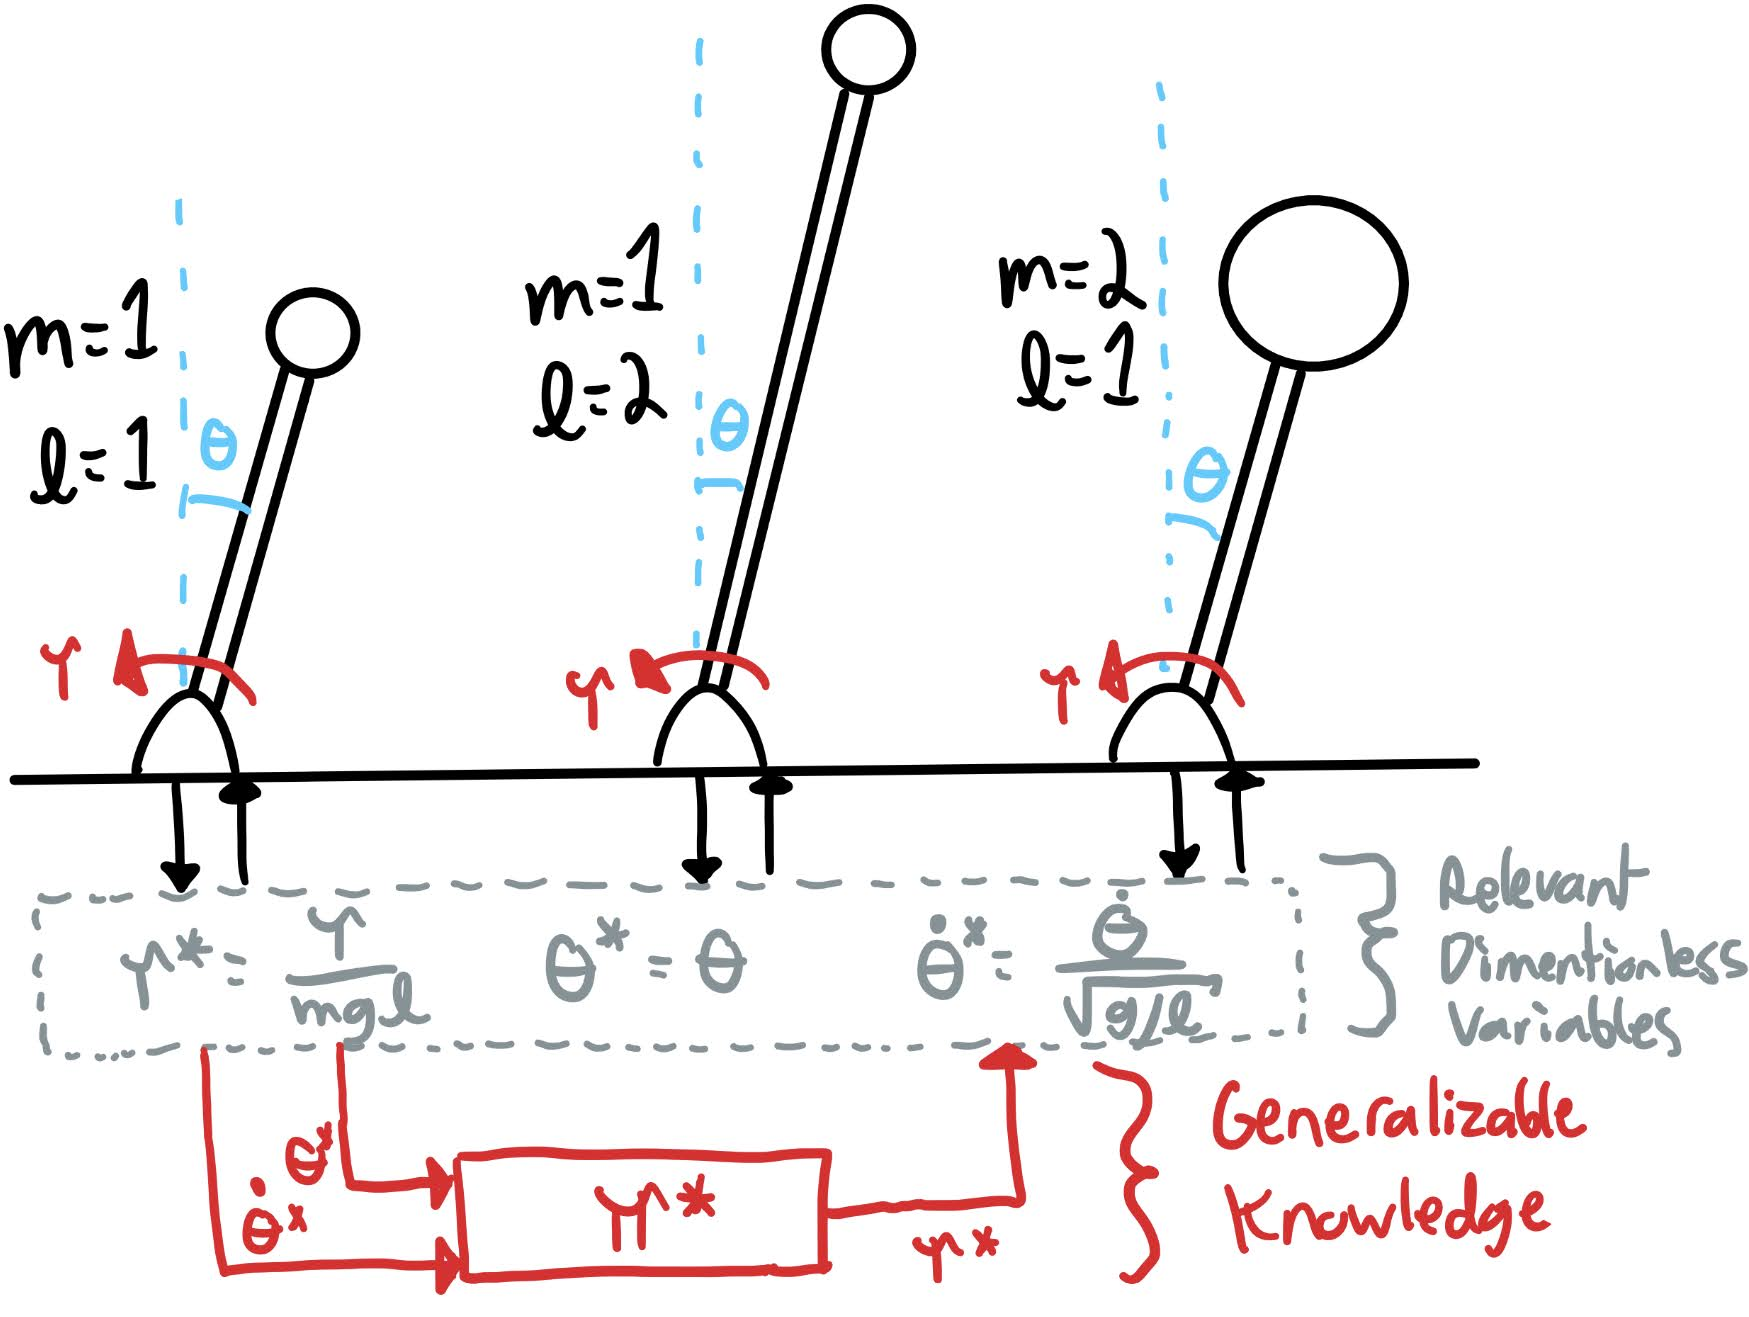
\includegraphics[width=0.99\linewidth]{fig/bigpicture2.jpg}
\caption{Big picture}\label{fig:big_picture}
\end{center}
\vspace{-25pt}
\end{figure}
%%%%%%%%%%%%%%%%%%%%%%


The context $c$ is the vector of all variables that would affect what is the feedback law solution to a motion control problem. For instance, in section \ref{sec:optimalswingup}, a case study is conducted considering the optimal feedback law for swinging-up an inverted pendulum. For this exemple, the context variables are the pendulum mass $m$, the gravitational constant $g$, the lenght $l$, but also what we will call task parameters: a parameter in the cost function $q$ and a constraint $\tau_{max}$ on the maximum input torque, see Fig. \ref{fig:policy_context}. For a given state of the system, the torque solution might be different if any of the context variable is modify, for instance if the pendulum is heavier, more torque limited, etc.
%%%%%%%%%%%%%%%%%%%%%%
\begin{figure}[h]
\vspace{-5pt}
\begin{center}
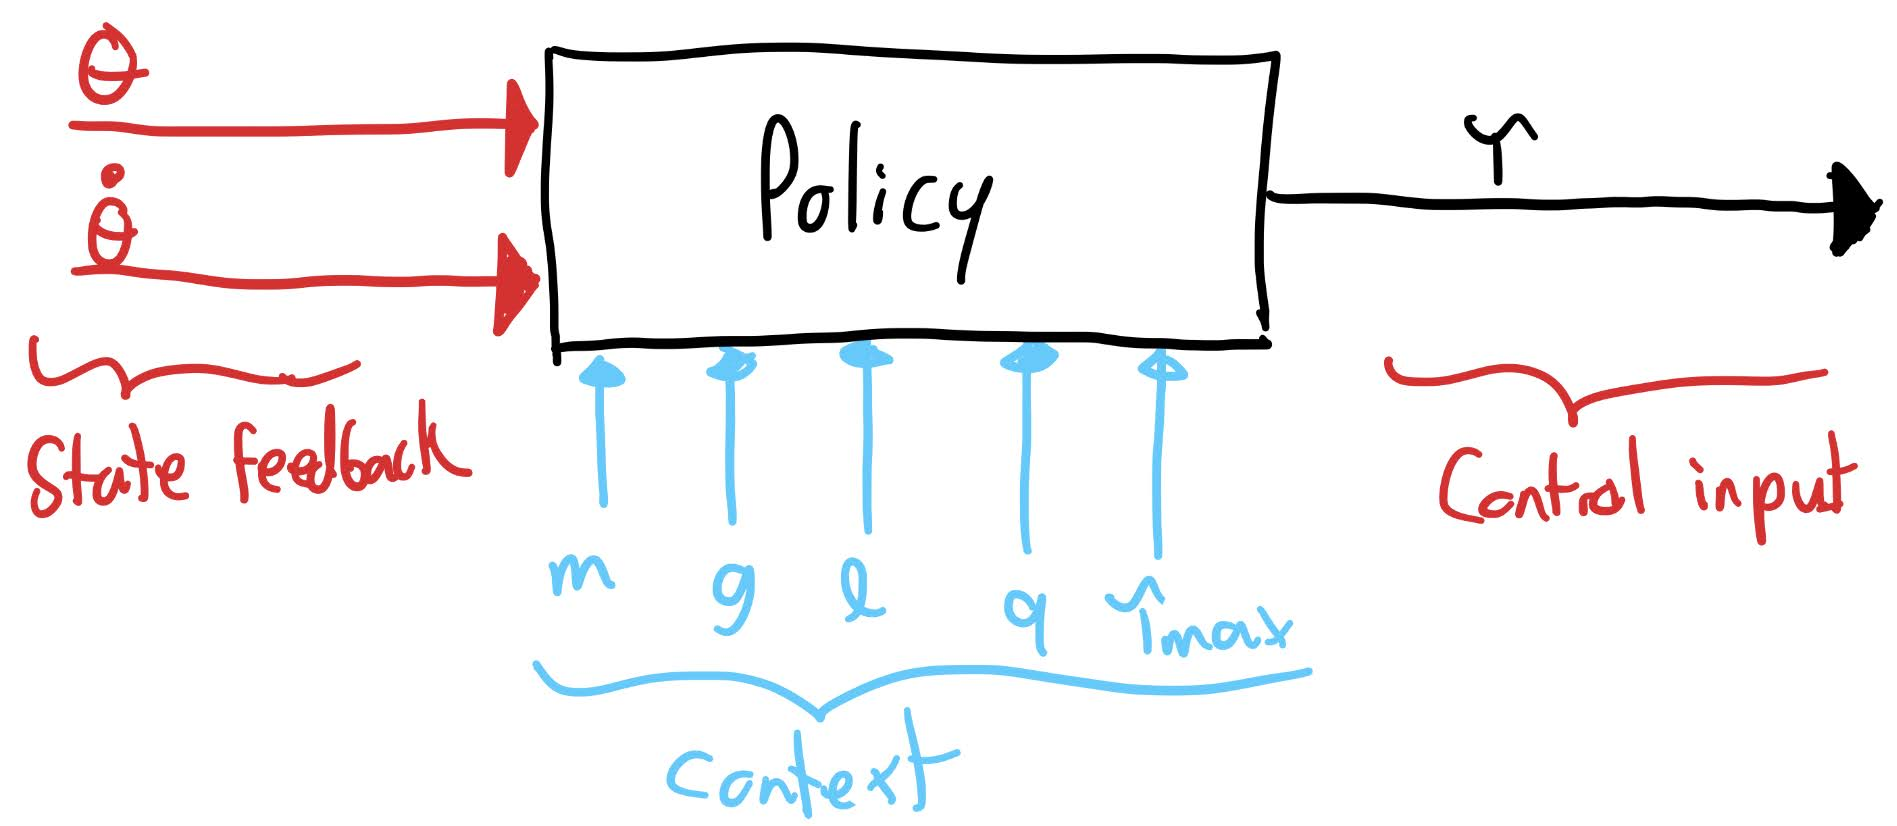
\includegraphics[width=0.95\linewidth]{fig/policy_context.jpg}
\caption{For the pendulum swing-up task, the context is 5 variables: the parameter of the system: $m$, $g$, and $l$, a parameter of the cost function: $q$ and a parameter defining the constraints: $\tau_{max}$. The feedback law solution i
}\label{fig:policy_context}
\end{center}
\vspace{-5pt}
\end{figure}
%%%%%%%%%%%%%%%%%%%%%%

 The context must include all the variables, system parameters and task parameters, that would affect the solution to the control problem:
%%%%%%%%%%%%%%%%%%%%%%
\begin{equation}
\underbrace{\begin{bmatrix}
u_1 \\
\vdots \\
u_k
\end{bmatrix}}_{\text{inputs}}
=
\pi \left(
\underbrace{\begin{bmatrix}
x_1 \\
\vdots \\
x_n
\end{bmatrix}}_{\text{states}}
,
\underbrace{
\underbrace{\begin{bmatrix}
c_1 \\
\vdots \\
\vdots \\
c_m
\end{bmatrix}}_{\text{system}}
,
\underbrace{\begin{bmatrix}
c_{m+1} \\
\vdots \\
c_{m+l}
\end{bmatrix}}_{\text{task}}
}_{\text{Context $c$}}
\right) 
\label{eq:vectorpolicy}
\end{equation}
%%%%%%%%%%%%%%%%%%%%%%


Then we can formalize the goal of generalizing a policy to a different context: if a good feedback policy $f_a$ is found for a system in a context $a$ described by variables $c_a$, can this knowledge help finding an equivalent good feedback policy in a different context $c_b$?
%%%%%%%%%%%%%%%%%%%%%%
\begin{equation}
\pi \left(
x,
c = c_a
\right) = 
f_a \left(
x 
\right) 
\quad \Rightarrow \quad
\pi \left(
x,
c = c_b
\right) = ?
\end{equation}
%%%%%%%%%%%%%%%%%%%%%%
Using the Buckinham Pi theorem [Cite something], we will show that if a dimentionless version of the context is equal, then a dimentionless version of the policy mapping must be also equivalent.


% %%%%%%%%%%%%%%%%%%%%%%
% \begin{figure}[H]
% \begin{center}
% 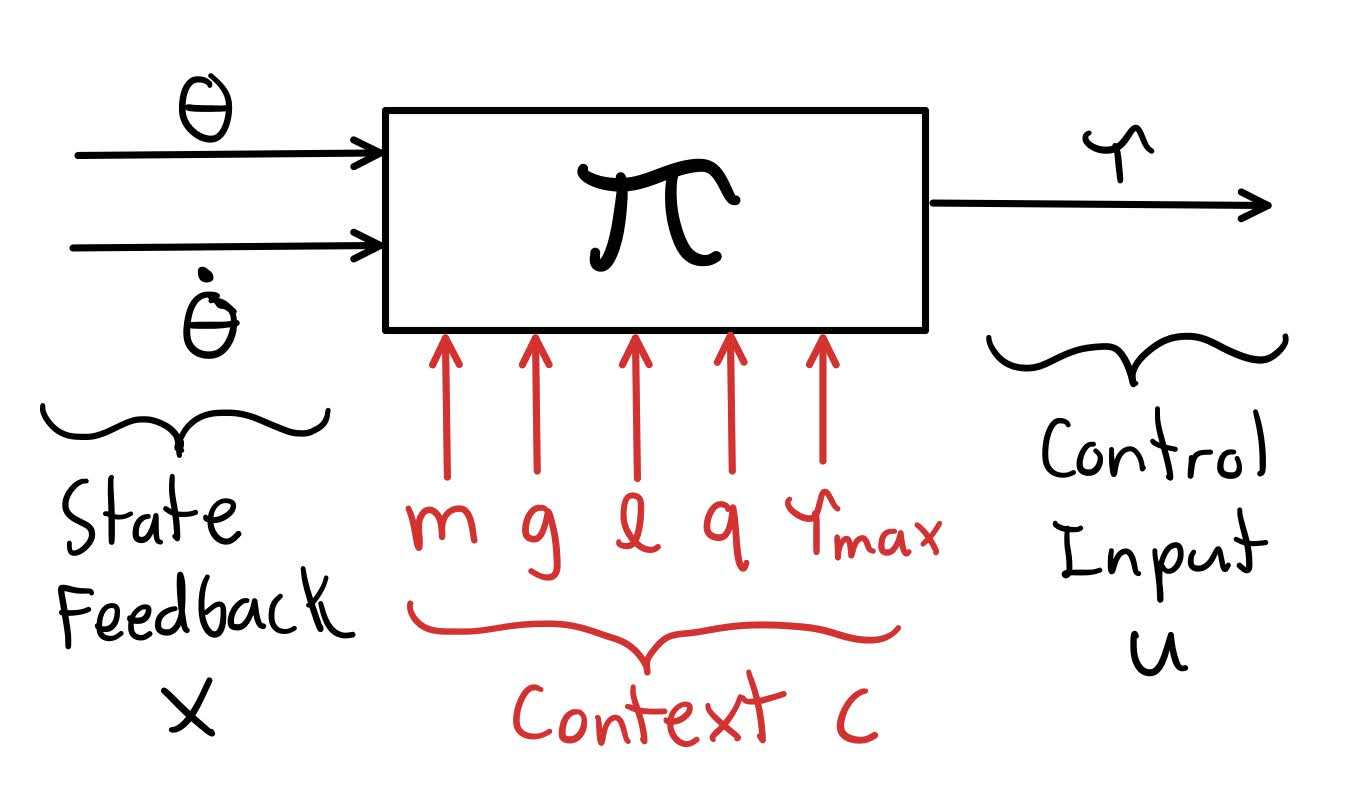
\includegraphics[width=0.99\linewidth]{fig/policy_context2.jpg}
% \caption{Big picture}\label{fig:policy_context}
% \end{center}
% \end{figure}
% %%%%%%%%%%%%%%%%%%%%%%

\subsection{Dimentional analysis of the augmented policy mapping}

For a system with $k$ control inputs, we can treat the augmented policy as $k$ mappings from states and context variables to each scalar control input $u_j$:
%%%%%%%%%%%%%%%%%%%%%%
\begin{equation}
u_j = \pi_j \left(
x_1, \hdots, x_n, 
c_1, \hdots \hdots, c_{m+l}
\right) 
\label{eq:scalarpolicy}
\end{equation}
%%%%%%%%%%%%%%%%%%%%%%
% %%%%%%%%%%%%%%%%%%%%%%
% \begin{equation}
% u_j = \pi_j \left(
% x,
% c 
% \right) \quad j = \{ 1, \hdots , k \}
% \end{equation}
% %%%%%%%%%%%%%%%%%%%%%%
where eq. \eqref{eq:scalarpolicy} is the $j$th line of the policy in vector form described by eq. \eqref{eq:vectorpolicy}.
Then, if the state vector is define by $n$ variables, and the context is defined by $m$ system parameters plus $l$ tasks parameters, then each mapping $\pi_j$ involves $1 + n + m + l$ (usually dimentionnal) variables. Here, we will assume that the policy fonction is physically meaningful, in the sense of the requirement for applying the Buckingham Pi theorem [Cite]. This means for exemple, that a policy that compute a force based on position and velocity measurement would be in this framework, but not of policy for playing chess for instance. 

Applying the Buckingham Pi theorem to the relashionship, tell us that if $d$ dimensions are involved in all thoses variables, then \ref{eq:scalarpolicy} can be restated into an equivalent dimentionless relationship between $p$ dimentionless $\Pi$ groups where $p \geq (1 + n + m + l ) - d$ [cite bukhingham pi]. Assuming $d$ dimentions are involved in the $m$ system parameter, and that we are in a situation where the maximum reduction is possible $p = (1 + n + m + l ) - d$, we can pick $d$ context variable $\{c_1, c_2 , \hdots,c_d\}$ as the basis (the repeated variables) to scale all other variables in a dimentionless form (we will note dimentionless $\Pi$ group as variables with an ${}^*$ subscript):
%%%%%%%%%%%%%%%%%%%%%%
\begin{align}
u_j^* &= u_j \left[ c_1 \right]^{e^u_{1j}} \left[ c_2 \right]^{e^u_{2j}} \hdots \left[ c_d \right]^{e^u_{dj}} \quad \scriptstyle j = \{ 1, \hdots , k \} \label{eq:piu}\\
x_i^* &= x_i \left[ c_1 \right]^{e^x_{1i}} \left[ c_2 \right]^{e^x_{2i}} \hdots \left[ c_d \right]^{e^x_{di}} \quad \scriptstyle i = \{ 1, \hdots , n \} \label{eq:pix}\\
c_i^* &= c_i\left[ c_1 \right]^{e^c_{1i}} \left[ c_2 \right]^{e^c_{2i}} \hdots \left[ c_d \right]^{e^c_{di}} \quad \scriptstyle i = \{ d+1, \hdots , m+l \} \label{eq:pic}%\\
%b_i^* &= b_i \left[ a_1 \right]^{e_1} \left[ a_2 \right]^{e_2} \hdots \left[ a_d \right]^{e_d} \quad  i = \{ 1, \hdots , l \} 
\end{align}
%%%%%%%%%%%%%%%%%%%%%%
where exposant $e$ are rational numbers selected to make all equations dimentionless. Then, the buckingham theorem tell us that the relationship described by eq. \eqref{eq:scalarpolicy} can be restated as the following relationship between  dimentionsless variables:
%%%%%%%%%%%%%%%%%%%%%%
\begin{equation}
u_j^* = \pi_j^* \left(
x_1^*, \hdots, x_n^*, 
c_{d+1}^*, \hdots, c_{m+l}^*, 
%b_1^*, \hdots, b_l^*, 
\right) 
\label{eq:scalardimpolicy}
\end{equation}
%%%%%%%%%%%%%%%%%%%%%%
involving $d$ less dimentionless variables in eq. \eqref{eq:scalarpolicy}. If we apply the same procedure to all control inputs, when can then assemble the $k$ mapping back into a vector form:
%%%%%%%%%%%%%%%%%%%%%%
\begin{equation}
\underbrace{
\begin{bmatrix}
u_1^* \\
\vdots \\
u_k^*
\end{bmatrix}
=
\pi^* \Biggl(
\begin{bmatrix}
x_1^* \\
\vdots \\
x_n^*
\end{bmatrix}
}_{\text{Dimentionless feedback law $f^*$}}
,
\underbrace{
\begin{bmatrix}
c_{d+1}^* \\
\vdots \\
c_{m}^*
\end{bmatrix}
,
\begin{bmatrix}
c_{m+1}^* \\
\vdots \\
c_{m+l}^*
\end{bmatrix}
}_{\text{Dimentionless context $c^*$}}
\Biggr)
\label{eq:vectordimpolicy}
\end{equation}
%%%%%%%%%%%%%%%%%%%%%%
that we will sometime write in compact form as: 
%%%%%%%%%%%%%%%%%%%%%%
\begin{equation}
u^* = \pi^*( x^* , c^* )
\label{eq:vectordimpolicyshort}
\end{equation}
%%%%%%%%%%%%%%%%%%%%%%

One interesting perk of this dimentional analysis, is that we can remove $p$ variables form the context (typically $p$ would be 2 or 3 for controlling a physical system involving time, force and length). The global problem of learning $\pi(x,c)$, i.e. the good feeback policy for all possible context is thus simplified in a dimentionless form. Also, an even more interesting feature, that we can use for transfering feedback law between systems, is that a global policy $\pi( x , c )$, will have an equivalent dimentionless form for multiple context $c$. As illustrated at Fig. \ref{fig:c_space}, the dimentionless context $c^*$ is a lower dimentional space ($m+l-d$) and multiple context vector $c$ will correspond to the same dimentionless vector $c^*$. 
%%%%%%%%%%%%%%%%%%%%%%
\begin{figure}[ht]
\vspace{-5pt}
\begin{center}
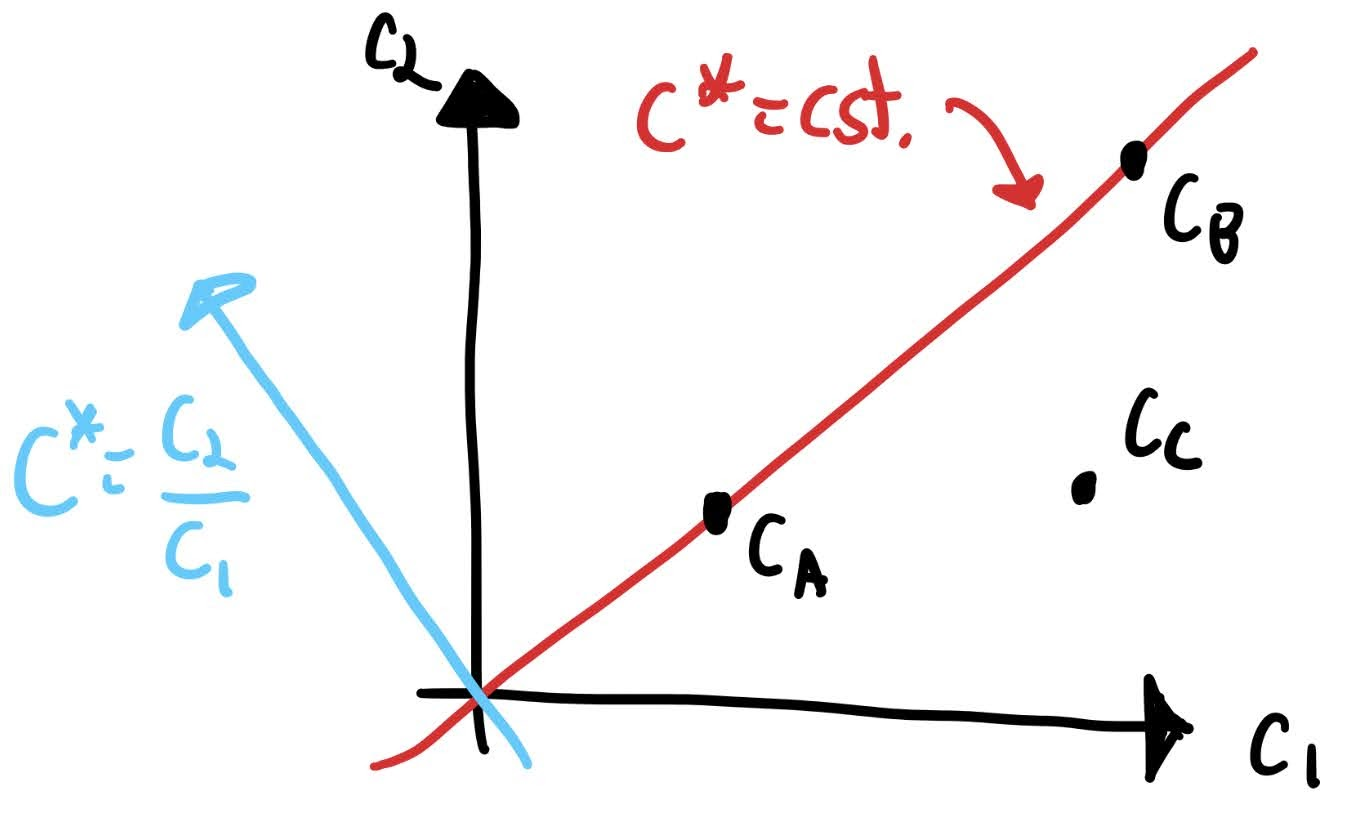
\includegraphics[width=0.80\linewidth]{fig/c_space.jpg}
\caption{Dimentionlaly similar context}\label{fig:c_space}
\end{center}
\vspace{-15pt}
\end{figure}
%%%%%%%%%%%%%%%%%%%%%%

For a given control problem, if the dimentionless context are equal, then the dimentionless feedback law should be eactly equivalent:
%%%%%%%%%%%%%%%%%%%%%%
\begin{equation}
\text{if} \quad c_a^* = c_b^*  \quad \text{then} \quad f_a^*(x^*) = f_b^*(x^*) \; \forall x^*   
\end{equation}
%%%%%%%%%%%%%%%%%%%%%%
where
%%%%%%%%%%%%%%%%%%%%%%
\begin{align}
f_a^*(x^*) = \pi^*( x^* , c^* = c_a^*)\\
f_b^*(x^*) = \pi^*( x^* , c^* = c_b^*)
\end{align}
%%%%%%%%%%%%%%%%%%%%%%
This is simply based on the fact that the dimentionless policy (eq. \eqref{eq:vectordimpolicyshort}) give the same output for the same inputs. This results means that the knowledge of a policy for a specific context $c$ can actually be generalized to a sub-space of all context for which the dimentionless context $c^*$ is equal.

Lets illustrate this with an example of a spherical submarine for witch we have an optimal policy of trust as a function of two context variables: the sphere radius and its velocity. The dimentionless policy would only be a function of a single dimentionless context variable: the Reynolds number, and would be the same for all submarines with the same Reynolds number. 

\subsection{Transfering policies between contexts}

In order to exploit this property, it is usefull to define transformation matrices based on scalar equations \eqref{eq:piu}, \eqref{eq:pix} and \eqref{eq:pic}:
%%%%%%%%%%%%%%%%%%%%%%
\begin{align}
u^* &= \left[ T_u(c) \right] \, u  \label{eq:Tu} \\
x^* &= \left[ T_x(c) \right] \, x \label{eq:Tx} \\
c^* &= \left[ T_c(c) \right] \, c \label{eq:Tc}
\end{align}
%%%%%%%%%%%%%%%%%%%%%%
where matrices $T_u$ and $T_x$ are square diagonal matrix, where each diagonal term is a multiplication of the first $d$ context variables ($\{c_1, c_2 , \hdots,c_d\}$) up to a rational power (found by applying the buckinghan pi theorem). Equations \eqref{eq:Tu} and \eqref{eq:Tx} are inversible (unless a context variable is equal to zero) and can be used to go back-and-forth between dimentional and dimentionless state and input variables. The matrix $T_c$ however have $d$ less row than columns and eq. \eqref{eq:Tc} is not inversible: for a given context $c$ there is only one dimentionless context $c^*$, however a dimentionless context $c^*$ correspond to multiple dimentional context $c$.

To summarize the dimentional analysis procedure, using the transformation matrices, if a dimentional feedback law $f_a$ for a context $c_a$ is known:
%%%%%%%%%%%%%%%%%%%%%%
\begin{align}
f_a ( x ) &= \pi \left( x, c = c_a \right)
\end{align}
%%%%%%%%%%%%%%%%%%%%%%
its representation in dimentionless form:
%%%%%%%%%%%%%%%%%%%%%%
\begin{align}
f_a^* ( x^* ) &= \pi \left( x^*, c^* = c_a^* )\right) 
\end{align}
%%%%%%%%%%%%%%%%%%%%%%
can be found by scaling the input and output of $f_a$ with $T_u$ and $T_x$:
%%%%%%%%%%%%%%%%%%%%%%
\begin{align}
f_a^* ( x^* ) &= T_u(c_a) 
\underbrace{
f_a \left(  
\underbrace{
T_x^{-1}(c_a) \; x^*
}_{x}
\right)
}_{u}
\label{eq:f2star}
\end{align}
%%%%%%%%%%%%%%%%%%%%%%
and the dimentionless context values $c^*_a$ can be found using eq. \eqref{eq:Tc}.
% %%%%%%%%%%%%%%%%%%%%%%
% \begin{align}
% c_a^* &= T_c( c_a ) \; c_a 
% \end{align}
% %%%%%%%%%%%%%%%%%%%%%%
Inversely, if we know a dimentionless feedback law $f_b^*$, matrices $T_u$ and $T_x$ can be used to scale it back to a specific context $c_b$:
%%%%%%%%%%%%%%%%%%%%%%
\begin{align}
f_b ( x ) &= T^{-1}_u(c_b) 
\underbrace{
f_b^* \left(  
\underbrace{
T_x(c_b) \; x
}_{x^*}
\right)
}_{u^*}
\label{eq:star2f}
\end{align}
%%%%%%%%%%%%%%%%%%%%%%
Thus, eq. \eqref{eq:f2star} and eq. \eqref{eq:f2star} can be used to take any context specific feedback law, finding its dimentionless form, and scale it back to a new context. In general, there is no guarantee that the behavior of the scaled feedback law in the new context will be similar to the behavior of the feedback law in the original context. However, if the dimentionless context are equal, then the behavior should be eactly equivalent, because the motion control problem was actually the same problem but scaled. For instance, lets suppose an optimal policy $f_a$ is known for a specific context $c_a$, then applying the scaled policy:
%%%%%%%%%%%%%%%%%%%%%%
\begin{align}
f_b ( x ) &= 
\left[ T^{-1}_u(c_b) 
T_u(c_a) \right] \,
f_a \left( 
\left[
T_x^{-1}(c_a) 
T_x(c_b)
\right] \,
x
\right)
\label{eq:ab_transform}
\end{align}
%%%%%%%%%%%%%%%%%%%%%%
on a system described by the context $c_b$ will be equaly equivalent (up to scaling factors) if 
%%%%%%%%%%%%%%%%%%%%%%
\begin{equation}
c_b^* =  T_c( c_b ) \; c_b  = T_c( c_a ) \; c_a = c_a^* 
\end{equation}
%%%%%%%%%%%%%%%%%%%%%%
In section \ref{sec:optimalswingup}, we show exemples of this results with numerical solution to dimentionnaly similar pendulum swing-up problems. 


%%%%%%%%%%%%%%%%%%%%%%
\begin{figure}[t]
\vspace{-5pt}
\begin{center}
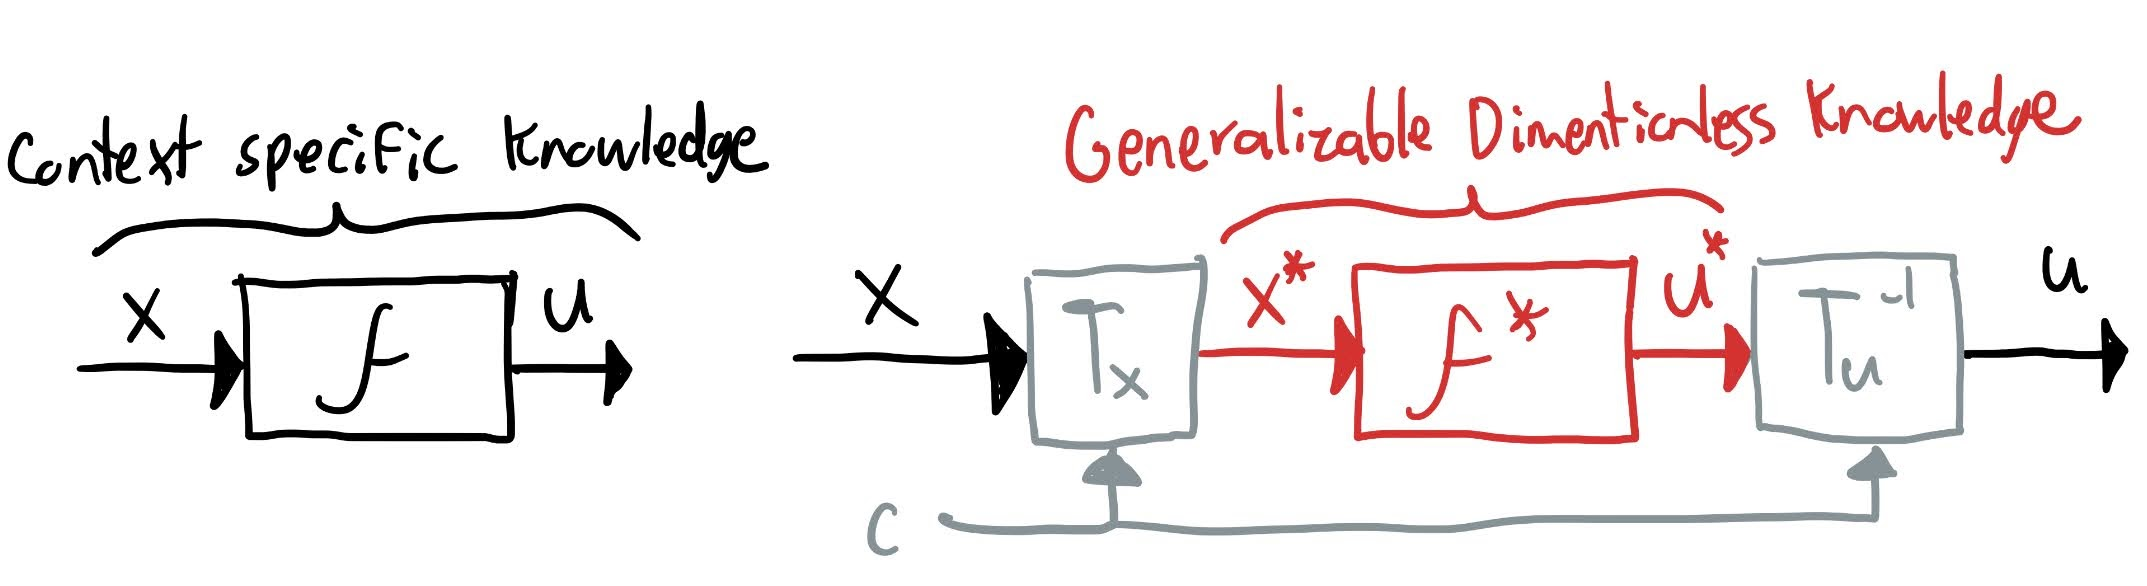
\includegraphics[width=0.99\linewidth]{fig/dimpol.jpg}
\caption{Isolating the dimentionless knowledge in a policy}\label{fig:dimpol}
\end{center}
\vspace{-15pt}
\end{figure}
%%%%%%%%%%%%%%%%%%%%%%



 







% %%%%%%%%%%%%%%%%%%%%%%
% \begin{equation}
% \underbrace{u}_{\text{inputs}}
% =
% \pi \left(
% \underbrace{x}_{\text{states}},
% \underbrace{\theta_s}_{\text{system parameters}},
% \underbrace{\theta_p}_{\text{policy parameters}}
% \right)
% \end{equation}
% %%%%%%%%%%%%%%%%%%%%%%


%%%%%%%%%%%%%%%%%%%%%%
\section{Optimal pendulum swing-up task}
\label{sec:optimalswingup}
In this paper, we will use a version of the pendulum swing-up task as a prototype problem to test the proposed ideas of dimentionless policies. The motion control problem is defined as finding a feedback law for controling the dynamic system is described by differential equations:
%%%%%%%%%%%%%%%%%%%%%%
\begin{equation}
ml^2 \ddot{\theta} - mgl \sin \theta = \tau
\label{eq:pendulum_dynamics}
\end{equation}
%%%%%%%%%%%%%%%%%%%%%%
that minimize the cost function given by:
%%%%%%%%%%%%%%%%%%%%%%
\begin{equation}
J = \int{( q^2 \theta^2 + 0 \, \dot{\theta}^2 + 1 \, \tau^2 ) dt }
\label{eq:pendulum_cost}
\end{equation}
%%%%%%%%%%%%%%%%%%%%%%
subject to input constraints given by:
%%%%%%%%%%%%%%%%%%%%%%
\begin{equation}
- \tau_{max} \leq \tau \leq \tau_{max}
\label{eq:pendulum_constraints}
\end{equation}
%%%%%%%%%%%%%%%%%%%%%%
Note that here, the cost function parameter $q$ is include in way to have units of torque, it was chosen to fixe the weight on velocity to zero for simplicity, and the weight on torque to one without loss of generality as only the relative value of weight with impact the solution. 

Thus, assuming there is no hidden variables and that equations \eqref{eq:pendulum_dynamics}, \eqref{eq:pendulum_cost} and \eqref{eq:pendulum_constraints} fully describe the problem. The solution, i.e. the optimal policy for all context, should be of the form given by:
%%%%%%%%%%%%%%%%%%%%%%
\begin{equation}
\underbrace{\tau}_{\text{inputs}}
=
\pi \left(
\underbrace{ \theta, \dot{\theta} }_{\text{states}},
\underbrace{
\underbrace{ m , g , l }_{\text{system parameters}},
\underbrace{ q , \tau_{max} }_{\text{task parameters}}
}_{\text{Context $c$}}
\right)
\end{equation}
%%%%%%%%%%%%%%%%%%%%%%
and involving variables listed in table \ref{tb:optimalswingup}.
%%%%%%%%%%%%%%%%%%%%%%%%%%%%%%%%%%%%%%%%%%%%
\begin{table}[htb]
   \centering % center the table
   \caption{Pendulum swing-up optimal policy variables} 
   \label{tb:optimalswingup}
   \begin{tabular}{p{0.8cm} p{2.5cm} p{0.8cm} p{1.5cm} }
   \hline \hline \noalign{\smallskip} \noalign{\smallskip} \noalign{\smallskip} \noalign{\smallskip}
   %%%%%%%%%%%%%%%%%%%%%%
   \textbf{Variable} & \textbf{Description} & \textbf{Units} & \textbf{Dimensions} \\ 
   %%%%%%%%%%%%%%%%%%%%%%
   \hline \hline \noalign{\smallskip} 
   \multicolumn{4}{c}{\textbf{Control inputs}}\\ \noalign{\smallskip}  \hline \hline
   \noalign{\smallskip} 
   %%%%%%%%%%%%%%%%%%%%%%
   $\tau$ & Actuator torque & $Nm$ & [$ML^2T^{-2}$]\\ 
   %%%%%%%%%%%%%%%%%%%%%%
   \hline \hline \noalign{\smallskip} 
   \multicolumn{4}{c}{\textbf{State variables}}\\ \noalign{\smallskip}  \hline \hline \noalign{\smallskip} 
   %%%%%%%%%%%%%%%%%%%%%%
   $\theta$ & Joint angle & $rad$ & []\\ \noalign{\smallskip} \hline \noalign{\smallskip}
   $\dot{\theta}$ & Joint angular velocity & $rad/sec$ & [$T^{-1}$] \\
   %%%%%%%%%%%%%%%%%%%%%%
   \hline \hline \noalign{\smallskip} 
   \multicolumn{4}{c}{\textbf{System parameters}}\\ \noalign{\smallskip}  \hline\hline  \noalign{\smallskip} 
   %%%%%%%%%%%%%%%%%%%%%%
   $m$ & Pendulum mass & $kg$ & [$M$]  \\ \noalign{\smallskip} \hline \noalign{\smallskip}
   $g$ & Gravity       & $m/s^2$ & [$LT^{-2}$]  \\ \noalign{\smallskip} \hline \noalign{\smallskip}
   $l$ & Pendulum lenght & $m$ & [$L$]  \\ \noalign{\smallskip} \hline \noalign{\smallskip}
%%%%%%%%%%%%%%%%%%%%%%
   \hline \hline \noalign{\smallskip} 
   \multicolumn{4}{c}{\textbf{Problem parameters}}\\ \noalign{\smallskip}  \hline\hline  \noalign{\smallskip} 
   %%%%%%%%%%%%%%%%%%%%%%
   $q$ & Weight parameter  & $Nm$ & [$ML^2T^{-2}$]   \\ \noalign{\smallskip} \hline \noalign{\smallskip}
   $\tau_{max}$ & Maximum torque & $Nm$ & [$ML^2T^{-2}$] \\ \noalign{\smallskip} \hline \noalign{\smallskip}
   \hline \noalign{\smallskip}
   %\bottomrule[\heavyrulewidth] 
   \end{tabular}
\end{table}
%%%%%%%%%%%%%%%%%%%%%%%%%%%%%%%%%%%%%%%%%%%%

Before, conducting the dimentional analysis, it is interesting to note that while there are 3 system paramters $m$, $g$ and $l$, they only appear indepedently in two groups in the dynamic equation. We can thus consider only two system parameters, and for convenience $mgl$ coresponding (the maximum static gravitationnal torque) and $\omega$ are selected, as listed at table \ref{tb:2param}

\begin{table}[htb]
   \centering % center the table
   \caption{Pendulum swing-up minimal system variables} 
   \label{tb:2param}
   \begin{tabular}{p{1.5cm} p{2.2cm} p{0.8cm} p{1.5cm} }
   \hline \hline \noalign{\smallskip} \noalign{\smallskip} 
   \multicolumn{4}{c}{\textbf{System parameters}}\\ \noalign{\smallskip}  \hline\hline  \noalign{\smallskip} 
   %%%%%%%%%%%%%%%%%%%%%%
   $mgl$ & Maximum gravitational torque  & $Nm$ & [$ML^2T^{-2}$]  \\ \noalign{\smallskip} \hline \noalign{\smallskip}
   $\omega = \sqrt{\frac{g}{l}}$ & Natural frequency & $sec^{-1}$ & [$T^{-1}$]  \\ \noalign{\smallskip} \hline \noalign{\smallskip}
   \hline \noalign{\smallskip}
   %\bottomrule[\heavyrulewidth] 
   \end{tabular}
\end{table}



% %%%%%%%%%%%%%%%%%%%%%%%%%%%%%%%%%%%%%%%%%%%%
% \subsection{Dimentionless dynamics}



% %%%%%%%%%%%%%%%%%%%%%%
% \begin{align}
% %ml^2 \ddot{\theta} + mgl \sin \theta &= \tau  \\
% \frac{\ddot{\theta}}{\omega^2} + \sin \theta &= \frac{\tau}{mgl}
% \end{align}
% %%%%%%%%%%%%%%%%%%%%%%

% %%%%%%%%%%%%%%%%%%%%%%
% \begin{equation}
% m = (n = 5 ) - ( p = 2 ) = 3
% \end{equation}
% %%%%%%%%%%%%%%%%%%%%%%

% %%%%%%%%%%%%%%%%%%%%%%
% \begin{align}
% \Pi_1 &= \tau^* = \frac{\tau}{mgl} \quad \quad \frac{[ML^2T^{-2}]}{[M][LT^{-2}][L]} \\
% \Pi_2 &= \theta^* = \theta \quad \quad [-]\\
% \Pi_3 &= \ddot{\theta}^* = \frac{ \ddot{\theta}  }{ \omega^2 } \quad \quad \frac{[T^{-2}]}{[T^{-1}][T^{-1}]} 
% \end{align}
% %%%%%%%%%%%%%%%%%%%%%%

% %%%%%%%%%%%%%%%%%%%%%%
% \begin{equation}
% \tau^*
% =
% f\left(
% \theta^*,\ddot{\theta}^*
% \right) = \ddot{\theta}^* + \sin \theta^*
% \end{equation}
% %%%%%%%%%%%%%%%%%%%%%%


\subsection{Dimentional analysis}

Here we have one control input, two state, two system parameter and two task parameter, for a total of $1+(n=2)+(m=2)+(l=2)=7$ variables are involved. In those variables, only $d=2$ independants dimensions ( $ML^2T^{-2}$ and $T^{-1}$ ) are present. Using $c_1 = mgl$ and $c_2 = \omega$ as the repeating variables leads to the following dimentionless groups:
%%%%%%%%%%%%%%%%%%%%%%
\begin{align}
\Pi_1 &= \tau^* = \frac{\tau}{mgl} \quad \quad \frac{[ML^2T^{-2}]}{[M][LT^{-2}][L]} \\
\Pi_2 &= \theta^* = \theta \quad \quad []\\
\Pi_3 &= \dot{\theta}^* = \frac{ \dot{\theta}  }{ \omega } \quad \quad \frac{[T^{-1}]}{[T^{-1}]} \\
\Pi_4 &= \tau_{max}^* = \frac{\tau_{max}}{mgl} \quad \quad \frac{[ML^2T^{-2}]}{[M][LT^{-2}][L]} \\
\Pi_5 &= q^* = \frac{q}{mgl} \quad \quad \frac{[ML^2T^{-2}]}{[M][LT^{-2}][L]} 
\end{align}
%%%%%%%%%%%%%%%%%%%%%%
Here, all 3 torque variables ($\tau$, $q$ and $\tau_{max}$) are scaled by the maximum gravitationnal torque, and the pendulum velocity variable is scaled by the pendulum natural frequency. The transformation matrices are then
%%%%%%%%%%%%%%%%%%%%%%
\begin{align}
\tau^* &= 
\underbrace{\left[  1/mgl \right]}_{T_u}
\, \tau  \label{eq:Tupendulum} \\
\begin{bmatrix}
\theta^* \\ \dot{\theta}^*
\end{bmatrix} &= 
\underbrace{
\begin{bmatrix}
    1 & 0 \\ 0 & 1/\omega
\end{bmatrix}
}_{T_x} \, 
\begin{bmatrix}
\theta \\ \dot{\theta}
\end{bmatrix}
 \label{eq:Txpendulum} \\
\begin{bmatrix}
q^* \\ \tau_{max}^*
\end{bmatrix} &= 
\underbrace{
\begin{bmatrix}
      1/mgl & 0 \\ 0 &  1/mgl
\end{bmatrix}
}_{T_c} \, 
\begin{bmatrix}
q \\ \tau_{max}
\end{bmatrix}
 \label{eq:Tcpendulum} 
\end{align}
%%%%%%%%%%%%%%%%%%%%%%
According to the theorem, any policy that is only based on the variable included in our analysis can be expressed as a relationship between the 5 dimentionless pi groups in the form:
%%%%%%%%%%%%%%%%%%%%%%
\begin{equation}
\tau^*
=
\pi^* \left(
\theta, \dot{\theta}^*,
q^* , \tau_{max}^* 
\right)
\end{equation}
%%%%%%%%%%%%%%%%%%%%%%

Here, the dimentional analysis shows that, for dimentionnally similar swing-up problem (which means here equal ratios $q^*$ and $\tau_{max}^*$) the optimal feedback laws should be equivalent in their dimentionless form. In other words, if we have an optimal policy $f_a$ found in a specific context $c_a = [m_a,l_a,g_a,q_a,\tau_{max,a}]$, and an optimal policy $f_b$ for a second context $c_b = [m_b,l_b,g_b,q_b,\tau_{max,b}]$. Then, both dimentionless form will be equal $f_a^*=f_b^*$ if $q^*_1 = q^*_2$ and $\tau_{max,1}^* = \tau_{max,2}^*$, what we call a \textit{dimentionnally similar context}. Furthermore, we can thus find $f_b$ using $f_a$ or vice-versa unsing the scaling given by eq. \eqref{eq:ab_transform}. However, if $q^*_a \neq q^*_b$ or $\tau_{max,a}^* \neq \tau_{max,b}^*$ then $f_a$ doesn't give us information on $f_b$ wihtout additionnal assumptions. 

%%%%%%%%%%%%%%%%%%%%%%
\subsection{Numerical results}

Here, a numerical algorithm (details of the methodology is presented at ...) is use to compute numerical solution to the prototype motion control problem defined by eq \eqref{eq:pendulum_dynamics}, \eqref{eq:pendulum_cost} and \eqref{eq:pendulum_constraints}. The used numerical recipe produce feedback law solution in the form of look-up table, based on the discretize grid of the state-space. 

The optimal (up to discretization error) feedback laws are computed for 9 contexts listed at table \ref{tb:9contexts}. In those 9 contexts, there is 3 sub-group of 3 cases with dimentionless similar context. Also each sub-group inlcude the same 3 pendulums, illustrated at Fig. \ref{fig:big_picture}, a regular, a twice longer and a twice heavier. Contexts 1, 2 and 3 describe a task where the torque is limited to half the satic maximum torque.  Contexts 4, 5 and 6 describe a task where the cost highly penalize applying large forces relatively to position errors. Contexts 7, 8 and 9 describe a task where the cost highly penalize position errors, relatively to applying large forces. 
%%%%%%%%%%%%%%%%%%%%%%%%%%%%%%%%%%%%%%%%%%%%
\begin{table}[htb]
   \centering % center the table
   \caption{Pendulum swing-up problems parameters} 
   \label{tb:9contexts}
   \begin{tabular}{ p{2.0cm} p{0.8cm} p{0.8cm} p{0.8cm} p{0.8cm} p{0.8cm} }
   \hline \hline \noalign{\smallskip} \noalign{\smallskip} 
   %%%%%%%%%%%%%%%%%%%%%%
      & $m$ & $g$ & $l$ & $q$ & $\tau_{max}$ \\ \hline
   %%%%%%%%%%%%%%%%%%%%%
   %%%%%%%%%%%%%%%%%%%%%%
   \hline \hline \noalign{\smallskip} 
   \multicolumn{6}{c}{\textbf{Problems with $\tau_{max}^* = 0.5$ and $q^* = 0.1$} }\\ \noalign{\smallskip}  \hline\hline  \noalign{\smallskip} 
   %%%%%%%%%%%%%%%%%%%%%%
   Context no 1 : & 1.0 & 10.0 & 1.0 & 1.0 & 5.0 \\
   Context no 2 : & 1.0 & 10.0 & 2.0 & 2.0 & 10.0 \\
   Context no 3 : & 2.0 & 10.0 & 1.0 & 2.0 & 10.0 \\
   %%%%%%%%%%%%%%%%%%%%%
   \hline \hline \noalign{\smallskip} 
   \multicolumn{6}{c}{\textbf{Problems with $\tau_{max}^* = 1.0$ and $q^* = 0.05$} }\\ \noalign{\smallskip}  \hline\hline  \noalign{\smallskip} 
   %%%%%%%%%%%%%%%%%%%%%%
   Context no 4 : & 1.0 & 10.0 & 1.0 & 0.5 & 10.0 \\
   Context no 5 : & 1.0 & 10.0 & 2.0 & 1.0 & 20.0 \\
   Context no 6 : & 2.0 & 10.0 & 1.0 & 1.0 & 20.0 \\
   %%%%%%%%%%%%%%%%%%%%%
   \hline \hline \noalign{\smallskip} 
   \multicolumn{6}{c}{\textbf{Problems with $\tau_{max}^* = 1.0$ and $q^* = 10$} }\\ \noalign{\smallskip}  \hline\hline  \noalign{\smallskip} 
   %%%%%%%%%%%%%%%%%%%%%%
   Context no 7 : & 1.0 & 10.0 & 1.0 & 100.0 & 10.0 \\
   Context no 8 : & 1.0 & 10.0 & 2.0 & 200.0 & 20.0 \\
   Context no 9 : & 2.0 & 10.0 & 1.0 & 200.0 & 20.0 \\
   %%%%%%%%%%%%%%%%%%%%%
   \hline \hline
   \end{tabular}
\end{table}
%%%%%%%%%%%%%%%%%%%%%%%%%%%%%%%%%%%%%%%%%%%%

Figure XXXX illustrate that for each sub-group with equal dimentionless context, the dimentional feedback law generated numerically, and also the exemple trajectory of the system starting from rest at the bottom position, looks very similar. They are similar up to a scaling of the axis, if we neglect slight differences due to discretization errors. Furthermore, when we compute the dimentionless verion of the feedback laws $f^*$, using eq. \eqref{eq:f2star}, the dimentionless version is actually equal within the dimentionaly similar context sub-group. This was the expected results given by the dimentional analysis of section \ref{sec:dimenanalysis}.



%%%%%%%%%%%%%%%%%%%%%%%%%%%%%%%%%%%%%%%%%%%%%%%%%%%
\subsection{Sensibility to context variables and regime}

%%%%%%%%%%%%%%%%%%%%%%
\begin{align}
\pi^*( \theta^* , \dot{\theta}^*, q^*, \tau_{max}^*) \approx 
\left\{
\begin{array}{c}
&f_{BB}^*( \theta^* , \dot{\theta}^* ) \; if \;  R^* \gg 1 \\
&f_{Tr}^*( \theta^* , \dot{\theta}^* ) \; if \;  R^* \approx 1\\
&f_{Un}^*( \theta^* , \dot{\theta}^* ) \; if \; R^* \ll 1
\end{array}
\right.
\end{align}
%%%%%%%%%%%%%%%%%%%%%%


%%%%%%%%%%%%%%%%%%%%%%
\begin{figure}[ht]
\begin{center}
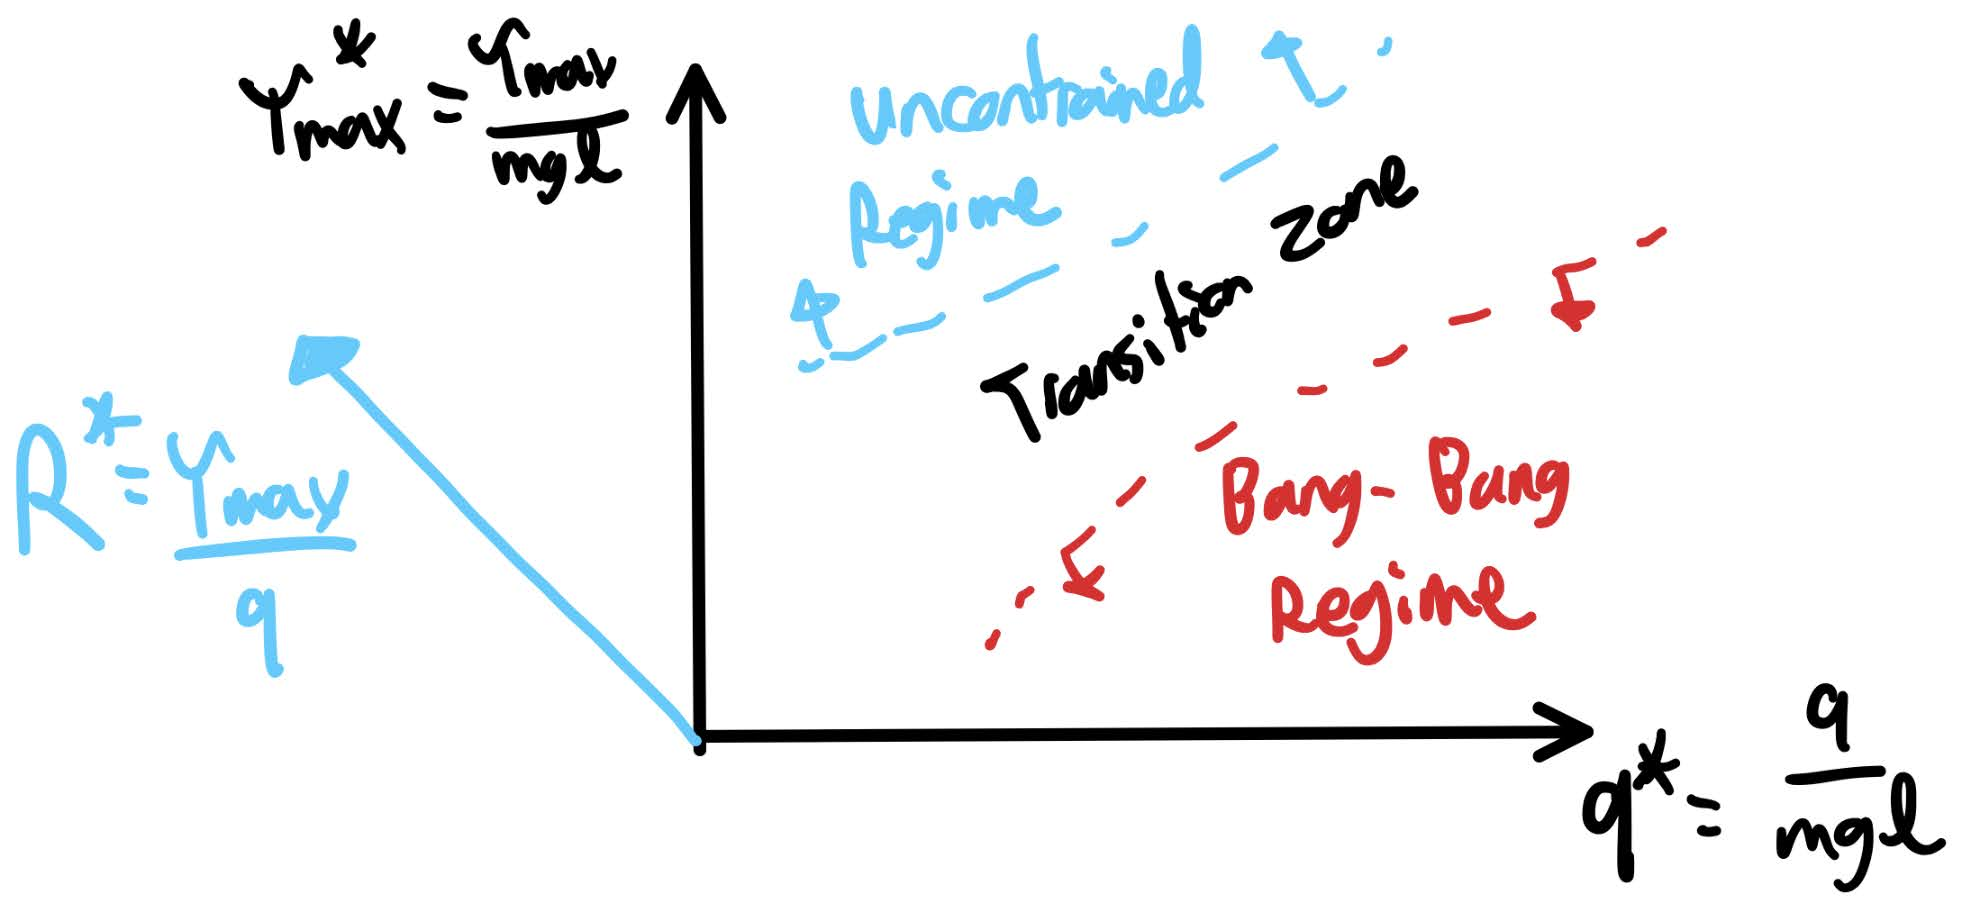
\includegraphics[width=0.99\linewidth]{fig/regimes.jpg}
\caption{Regime zones}\label{fig:regimeszones}
\end{center}
\end{figure}
%%%%%%%%%%%%%%%%%%%%%%

%%%%%%%%%%%%%%%%%%%%%%
\begin{figure}[ht]
\begin{center}
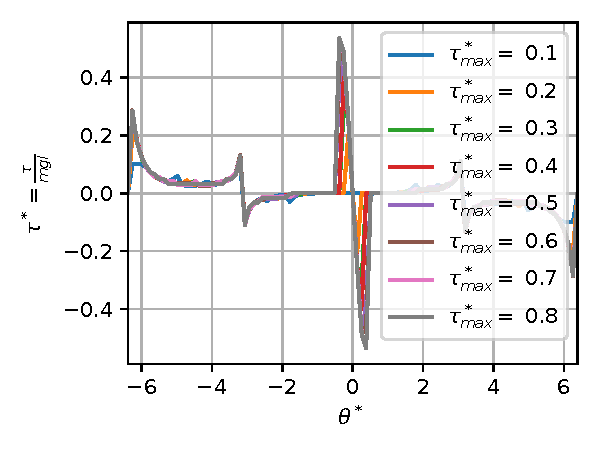
\includegraphics[width=0.99\linewidth]{fig/s_t_1_8.pdf}
\caption{Optimal dimentionless policy for various contexts $\tau^* = \pi^*( \theta^* , \dot{\theta}^* = 0 , q^* = 0.05 , \tau^*_{max} = [0.1, ... , 0.8] )$}\label{fig:regime}
\end{center}
\end{figure}
%%%%%%%%%%%%%%%%%%%%%%

% %%%%%%%%%%%%%%%%%%%%%%
% \begin{figure}[p]
% \begin{center}
% 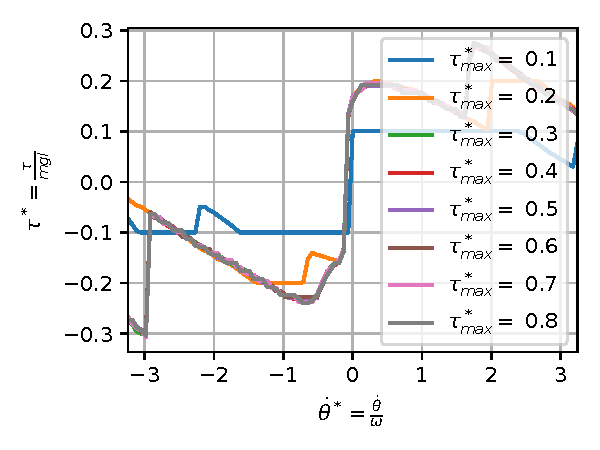
\includegraphics[width=0.99\linewidth]{fig/s_t_1_82.pdf}
% \caption{Optimal dimentionless policy for various contexts  $\tau^* = \pi^*( \theta^* = -\pi , \dot{\theta}^* , q^* = 0.05 , \tau^*_{max} )$}\label{fig:regime2}
% \end{center}
% \end{figure}
% %%%%%%%%%%%%%%%%%%%%%%

% %%%%%%%%%%%%%%%%%%%%%%
% \begin{figure}[p]
% \begin{center}
% 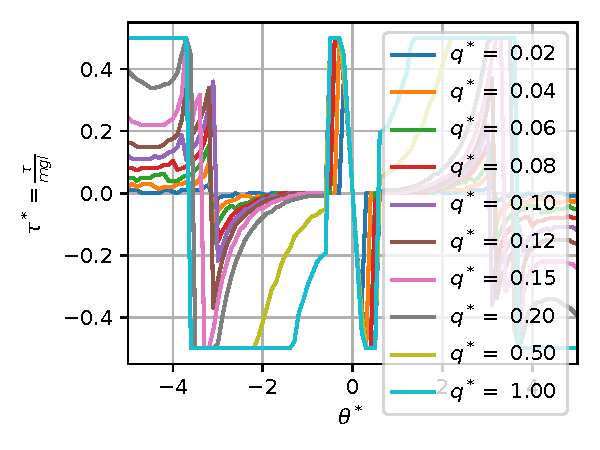
\includegraphics[width=0.99\linewidth]{fig/q_sensitivity.pdf}
% \caption{Optimal dimentionless policy for various contexts  $\tau^* = \pi^*( \theta^*  , \dot{\theta}^* = 0 , q^*  , \tau^*_{max} = 0.5 )$}\label{fig:q_sensitivity}
% \end{center}
% \end{figure}
% %%%%%%%%%%%%%%%%%%%%%%


%%%%%%%%%%%%%%%%%%%%%%
\begin{figure}[ht]
\begin{center}
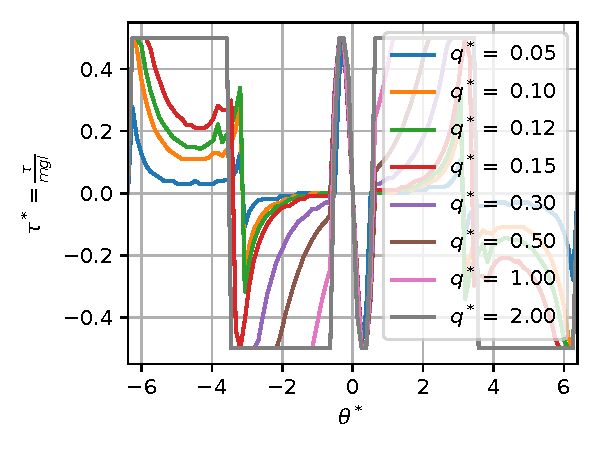
\includegraphics[width=0.99\linewidth]{fig/s_q_5_2.pdf}
\caption{Optimal dimentionless policy for various contexts  $\tau^* = \pi^*( \theta^*  , \dot{\theta}^* = 0 , q^* = [0.05, ... , 2.0]  , \tau^*_{max} = 0.5 )$}\label{fig:q_sensitivity}
\end{center}
\end{figure}
%%%%%%%%%%%%%%%%%%%%%%

% %%%%%%%%%%%%%%%%%%%%%%
% \begin{figure}[p]
% \begin{center}
% 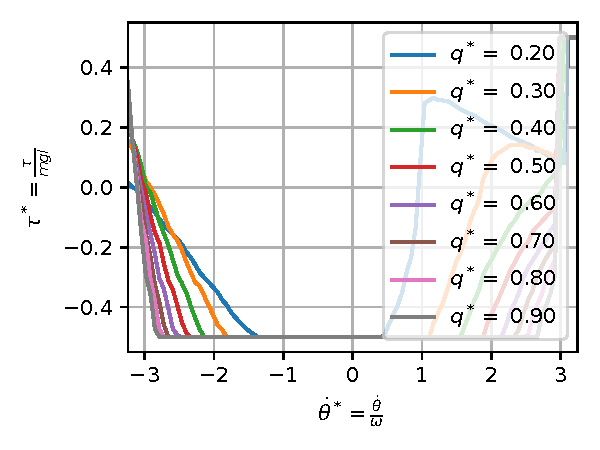
\includegraphics[width=0.99\linewidth]{fig/s_q_2_92.pdf}
% \caption{Optimal dimentionless policy for various contexts  $\tau^* = \pi^*( \theta^* = -\pi  , \dot{\theta}^*  , q^*  , \tau^*_{max} = 0.5 )$}\label{fig:q_sensitivity}
% \end{center}
% \end{figure}
% %%%%%%%%%%%%%%%%%%%%%%

% %%%%%%%%%%%%%%%%%%%%%%
% \begin{figure}[p]
% \begin{center}
% 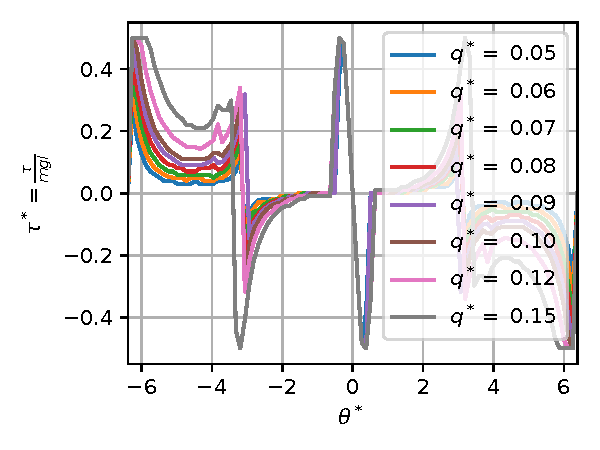
\includegraphics[width=0.99\linewidth]{fig/s_q_5_15.pdf}
% \caption{Optimal dimentionless policy for various contexts  $\tau^* = \pi^*( \theta^*  , \dot{\theta}^* = 0 , q^*  , \tau^*_{max} = 0.5 )$}\label{fig:q_sensitivity}
% \end{center}
% \end{figure}
% %%%%%%%%%%%%%%%%%%%%%%

% %%%%%%%%%%%%%%%%%%%%%%
% \begin{figure}[p]
% \begin{center}
% 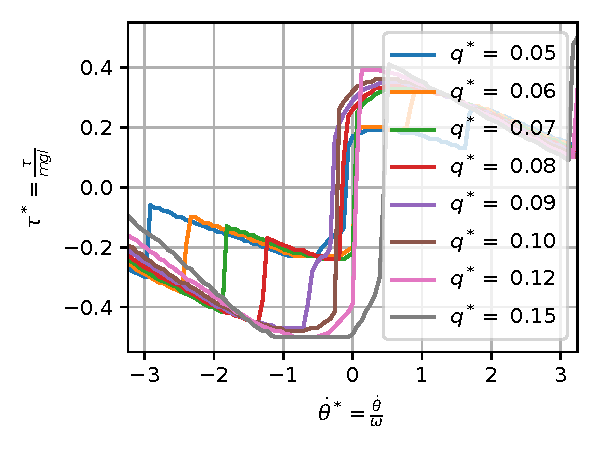
\includegraphics[width=0.99\linewidth]{fig/s_q_5_152.pdf}
% \caption{Optimal dimentionless policy for various contexts  $\tau^* = \pi^*( \theta^* = -\pi  , \dot{\theta}^*  , q^*  , \tau^*_{max} = 0.5 )$}\label{fig:q_sensitivity}
% \end{center}
% \end{figure}
% %%%%%%%%%%%%%%%%%%%%%%



%%%%%%%%%%%%%%%%%%%%%%%%%%%%%%%%%%%%%%%%%%%%%%%%%%%
\subsection{Trajectory solutions}

Trajectory solution are also generalizable


\subsection{Methodology}

We used the value-iteration [cite] algoithm on a discretized version of the continuous system...

\subsubsection{Additionnal dimentionless parameters for the solver}

Using dynamic programming for solving the optimal policy numerically require setting additionnal parameter that define the domain. Altough those parameter should not affect the optimal policy far away from the boundaries, here a dimensionless version of those parameters was kept fixed in all the experiments:
%%%%%%%%%%%%%%%%%%%%%%
\begin{align}
\theta^*_{max} &= \theta_{max} = 2 \pi \\
\dot{\theta}^*_{max} &= \frac{ \dot{\theta}_{max} }{\omega} = \pi \\
t^*_{f} &= t_{f} \; \omega = 10 \times 2 \pi 
\end{align}
%%%%%%%%%%%%%%%%%%%%%%
$\theta_{max}$ is the range of angle for witch the optimal policy is solved, here set at one full revolution. $\dot{\theta}_{max}$ is the range of angular velocity for witch the optimal policy is solved, here the dimentionless ratio scaled with the natural frequency is set at 2. $t_{f}$ is the time horizon, here its associated dimentionless ratio is fixed to always corespond to 10 periods of the pendulum using the natural frequency.



 \begin{figure*}[htp]
    \centering
    \vspace{-10pt}
    \subfloat[Feedback law $f$]{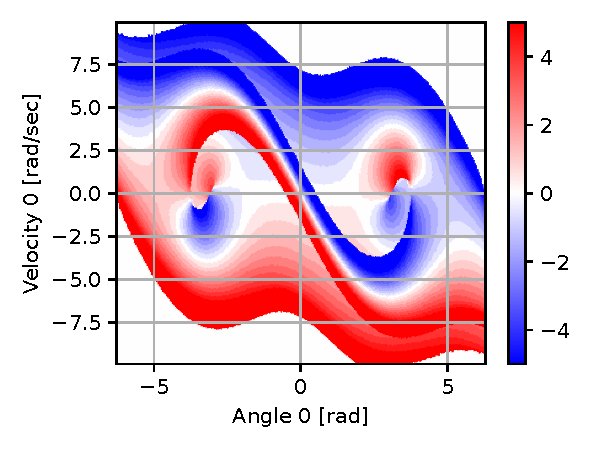
\includegraphics[width=0.33\textwidth]{fig/c1_policy.pdf}}
    \subfloat[Dimentionless feedback law $f^*$]{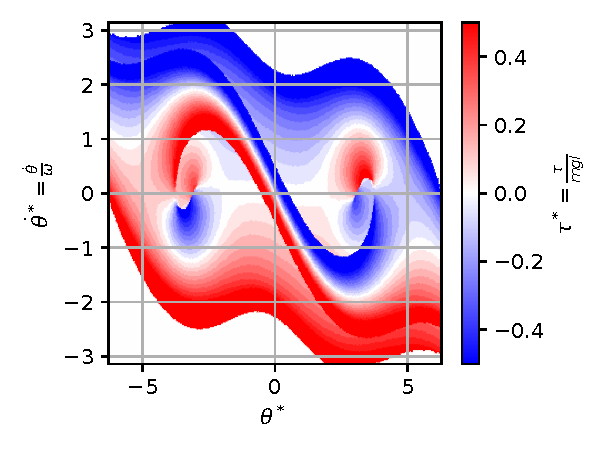
\includegraphics[width=0.33\textwidth]{fig/c1_dimpolicy.pdf}}   
    \subfloat[Exemple trajectory starting at $\theta=-\pi$]{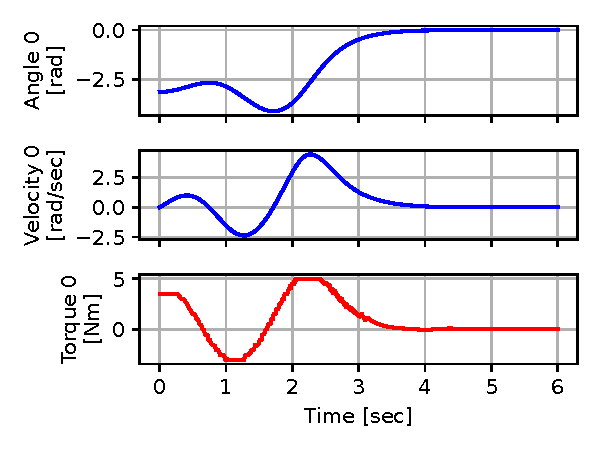
\includegraphics[width=0.33\textwidth]{fig/c1_traj.pdf}}
    \caption{Numerical results for context no 1}
    \label{fig:c1}
\end{figure*}

 \begin{figure*}[htp]
    \centering
    \vspace{-10pt}
    \subfloat[Feedback law $f$]{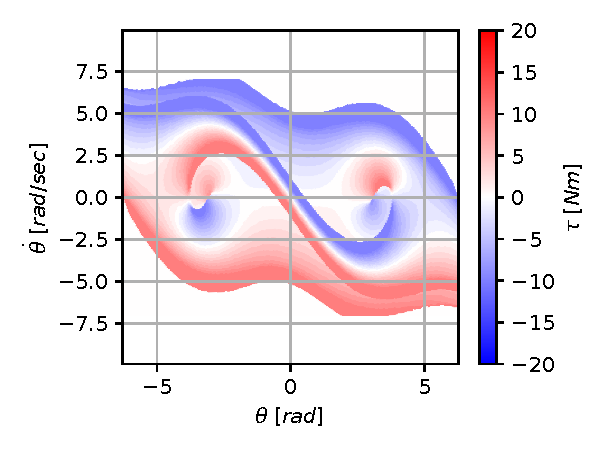
\includegraphics[width=0.33\textwidth]{fig/c2_policy.pdf}}
    \subfloat[Dimentionless feedback law $f^*$]{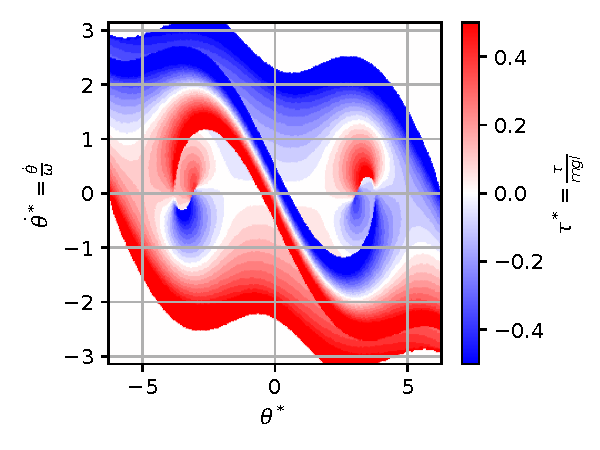
\includegraphics[width=0.33\textwidth]{fig/c2_dimpolicy.pdf}}   
    \subfloat[Exemple trajectory starting at $\theta=-\pi$]{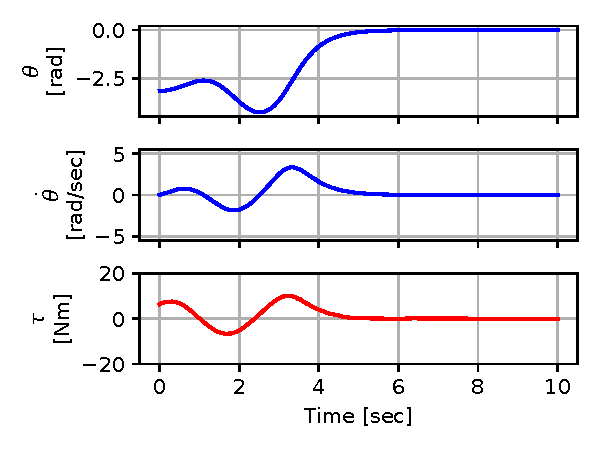
\includegraphics[width=0.33\textwidth]{fig/c2_traj.pdf}}
    \caption{Numerical results for context no 2}
    \label{fig:c2}
\end{figure*}

 \begin{figure*}[htp]
    \centering
    \vspace{-10pt}
    \subfloat[Feedback law $f$]{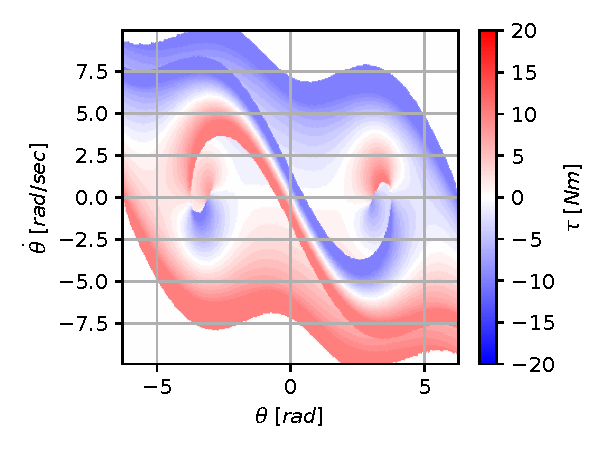
\includegraphics[width=0.33\textwidth]{fig/c3_policy.pdf}}
    \subfloat[Dimentionless feedback law $f^*$]{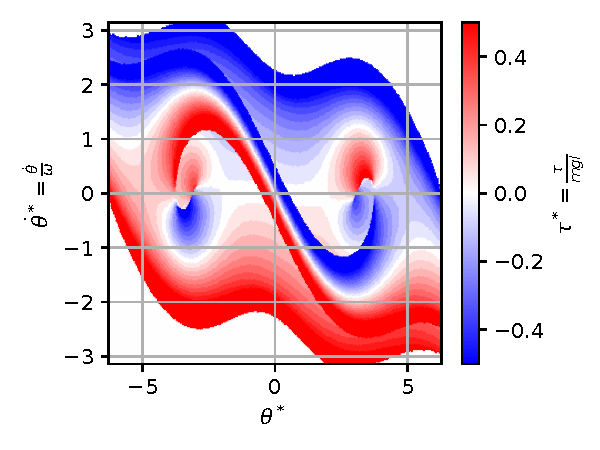
\includegraphics[width=0.33\textwidth]{fig/c3_dimpolicy.pdf}}   
    \subfloat[Exemple trajectory starting at $\theta=-\pi$]{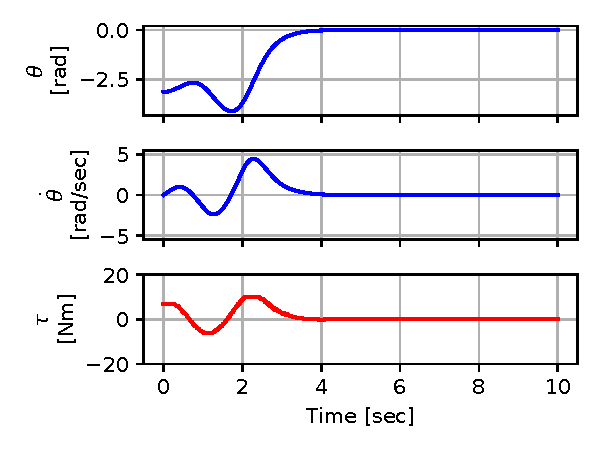
\includegraphics[width=0.33\textwidth]{fig/c3_traj.pdf}}
    \caption{Numerical results for context no 3}
    \label{fig:c3}
\end{figure*}

 \begin{figure*}[htp]
    \centering
    \vspace{-10pt}
    \subfloat[Feedback law $f$]{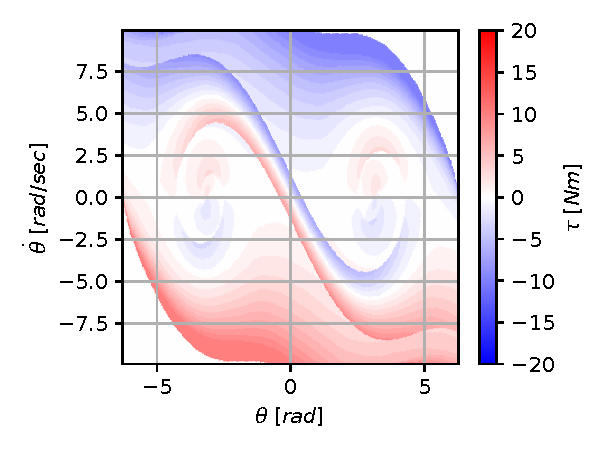
\includegraphics[width=0.33\textwidth]{fig/c4_policy.pdf}}
    \subfloat[Dimentionless feedback law $f^*$]{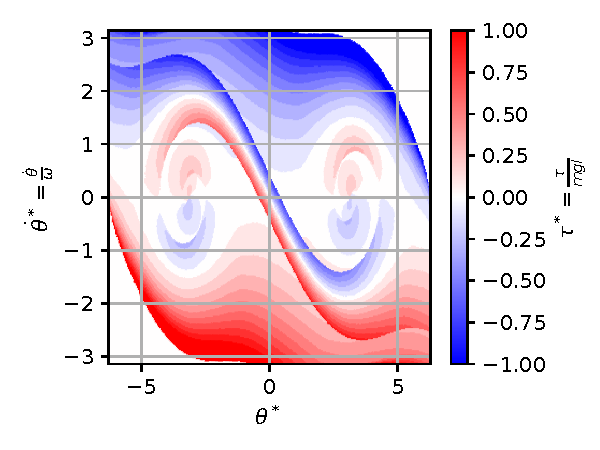
\includegraphics[width=0.33\textwidth]{fig/c4_dimpolicy.pdf}}   
    \subfloat[Exemple trajectory starting at $\theta=-\pi$]{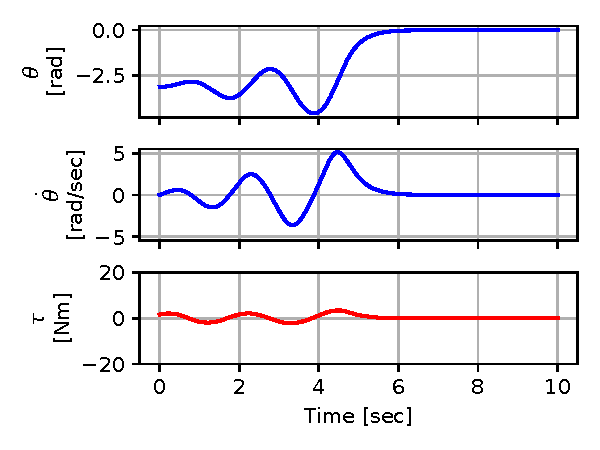
\includegraphics[width=0.33\textwidth]{fig/c4_traj.pdf}}
    \caption{Numerical results for context no 4}
    \label{fig:c4}
\end{figure*}

 \begin{figure*}[htp]
    \centering
    \vspace{-10pt}
    \subfloat[Feedback law $f$]{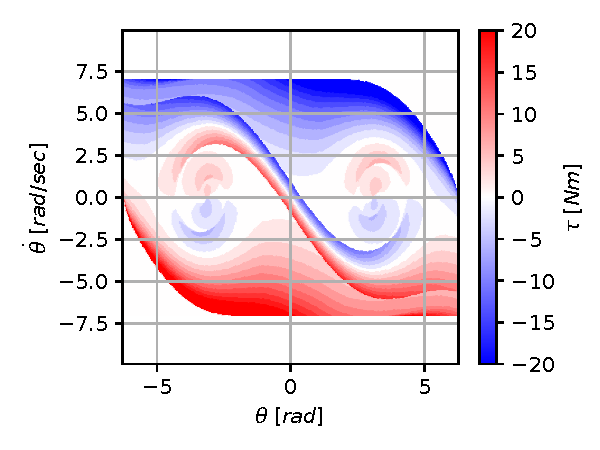
\includegraphics[width=0.33\textwidth]{fig/c5_policy.pdf}}
    \subfloat[Dimentionless feedback law $f^*$]{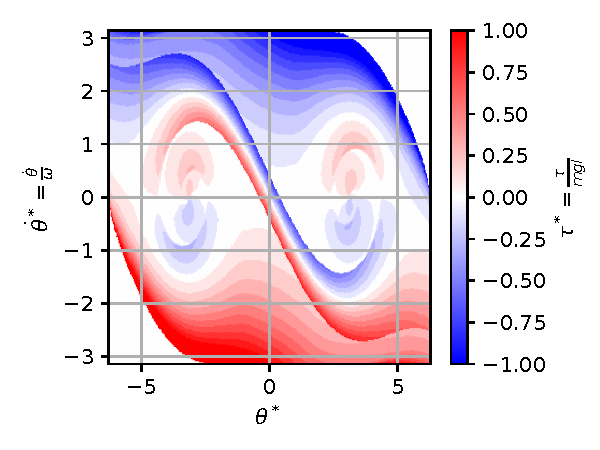
\includegraphics[width=0.33\textwidth]{fig/c5_dimpolicy.pdf}}   
    \subfloat[Exemple trajectory starting at $\theta=-\pi$]{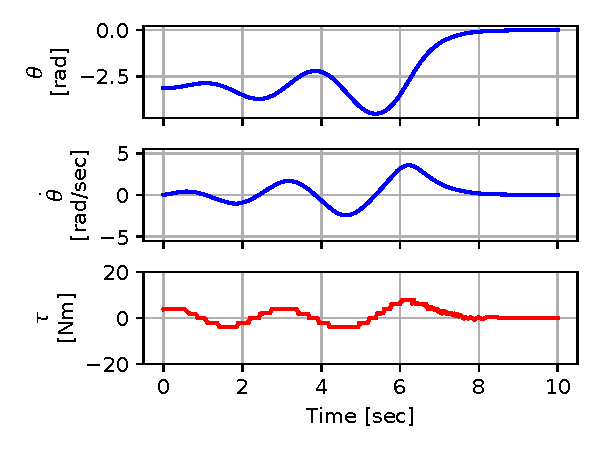
\includegraphics[width=0.33\textwidth]{fig/c5_traj.pdf}}
    \caption{Numerical results for context no 5}
    \label{fig:c5}
\end{figure*}

 \begin{figure*}[htp]
    \centering
    \vspace{-10pt}
    \subfloat[Feedback law $f$]{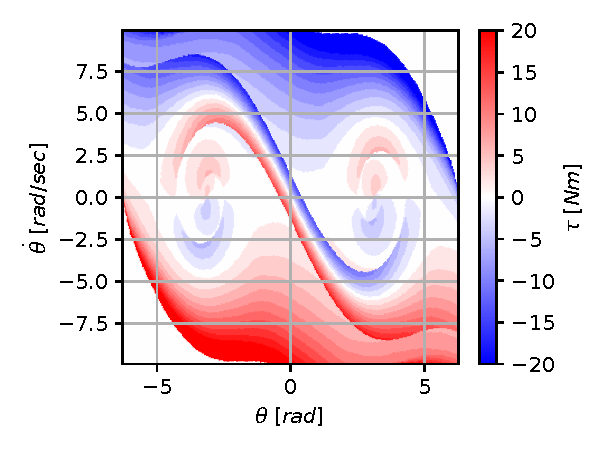
\includegraphics[width=0.33\textwidth]{fig/c6_policy.pdf}}
    \subfloat[Dimentionless feedback law $f^*$]{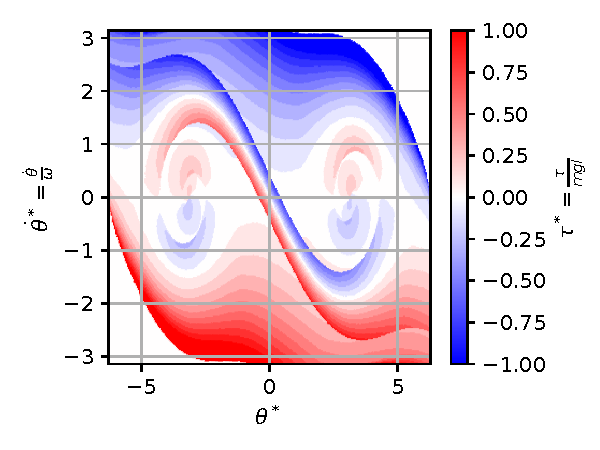
\includegraphics[width=0.33\textwidth]{fig/c6_dimpolicy.pdf}}   
    \subfloat[Exemple trajectory starting at $\theta=-\pi$]{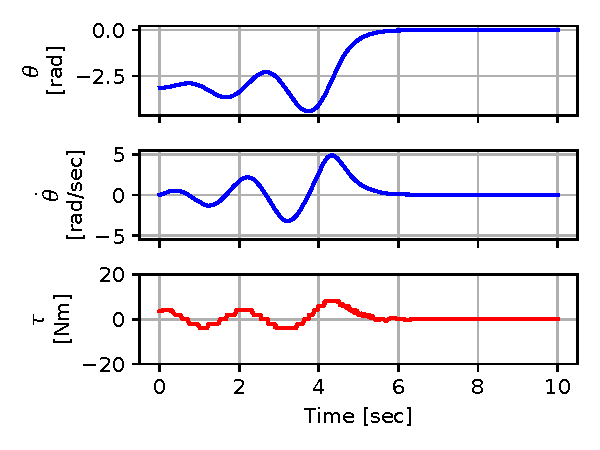
\includegraphics[width=0.33\textwidth]{fig/c6_traj.pdf}}
    \caption{Numerical results for context no 6}
    \label{fig:c6}
\end{figure*}

 \begin{figure*}[htp]
    \centering
    \vspace{-10pt}
    \subfloat[Feedback law $f$]{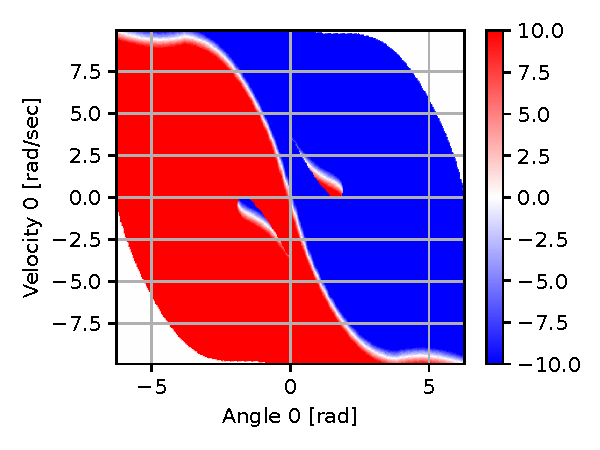
\includegraphics[width=0.33\textwidth]{fig/c7_policy.pdf}}
    \subfloat[Dimentionless feedback law $f^*$]{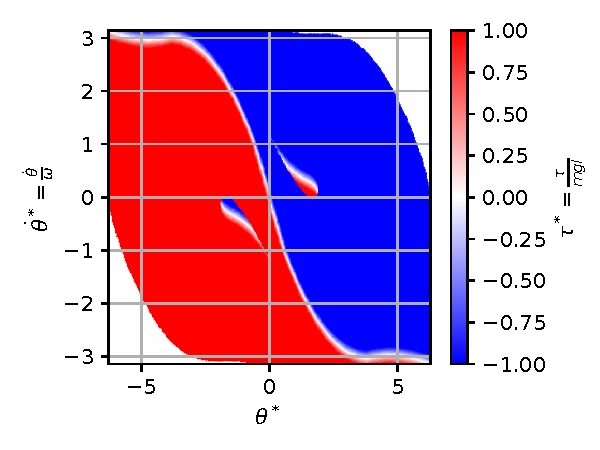
\includegraphics[width=0.33\textwidth]{fig/c7_dimpolicy.pdf}}   
    \subfloat[Exemple trajectory starting at $\theta=-\pi$]{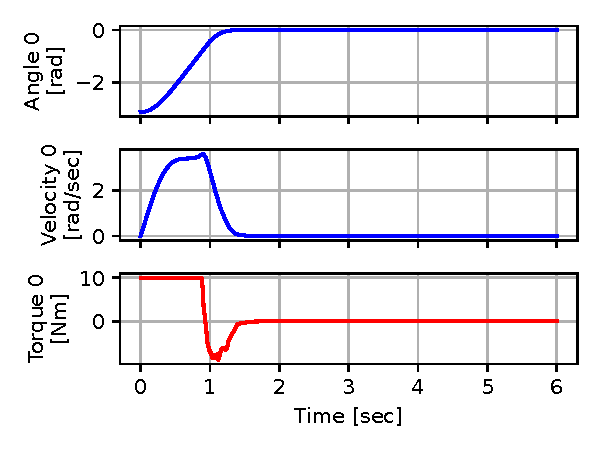
\includegraphics[width=0.33\textwidth]{fig/c7_traj.pdf}}
    \caption{Numerical results for context no 7}
    \label{fig:c7}
\end{figure*}

 \begin{figure*}[htp]
    \centering
    \vspace{-10pt}
    \subfloat[Feedback law $f$]{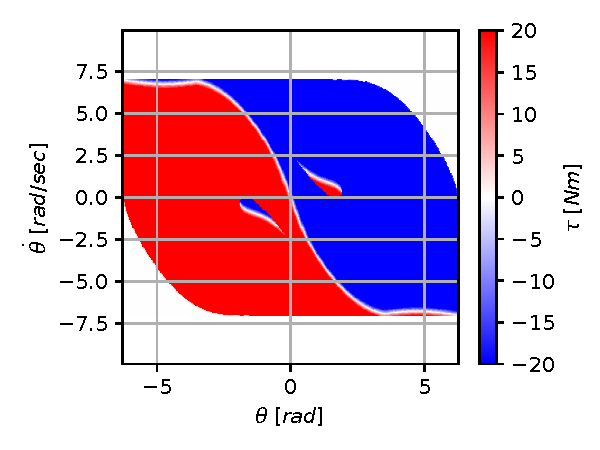
\includegraphics[width=0.33\textwidth]{fig/c8_policy.pdf}}
    \subfloat[Dimentionless feedback law $f^*$]{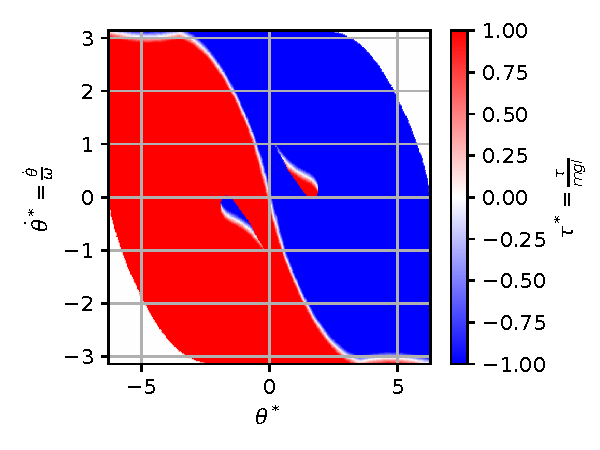
\includegraphics[width=0.33\textwidth]{fig/c8_dimpolicy.pdf}}   
    \subfloat[Exemple trajectory starting at $\theta=-\pi$]{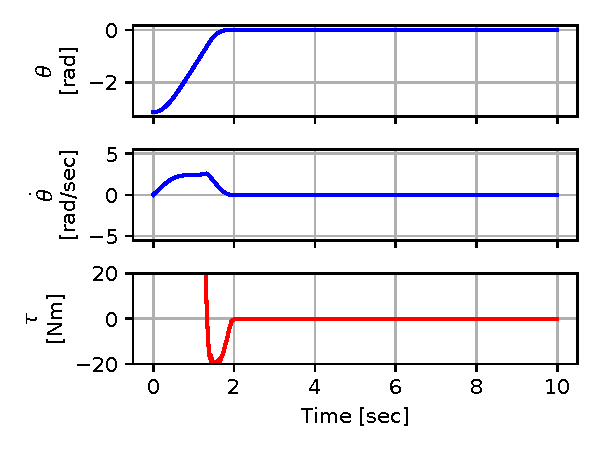
\includegraphics[width=0.33\textwidth]{fig/c8_traj.pdf}}
    \caption{Numerical results for context no 8}
    \label{fig:c8}
\end{figure*}

 \begin{figure*}[htp]
    \centering
    \vspace{-10pt}
    \subfloat[Feedback law $f$]{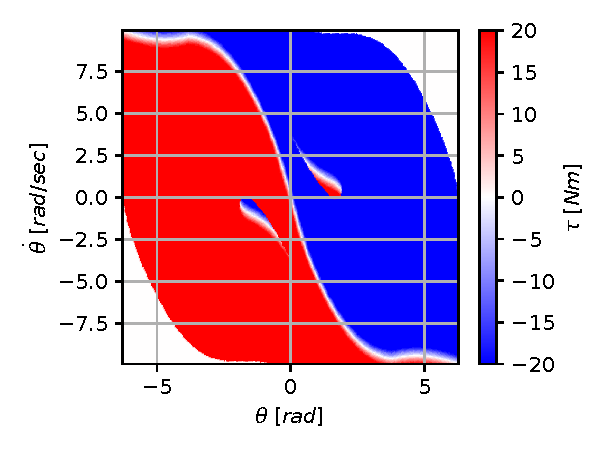
\includegraphics[width=0.33\textwidth]{fig/c9_policy.pdf}}
    \subfloat[Dimentionless feedback law $f^*$]{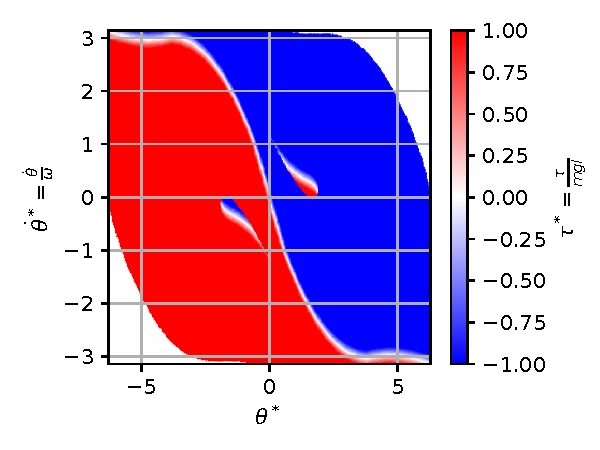
\includegraphics[width=0.33\textwidth]{fig/c9_dimpolicy.pdf}}   
    \subfloat[Exemple trajectory starting at $\theta=-\pi$]{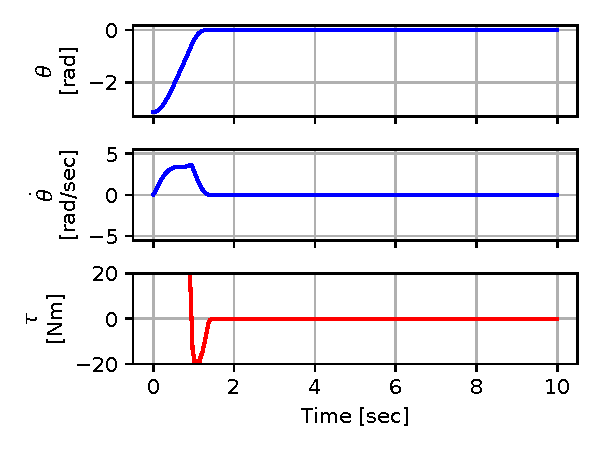
\includegraphics[width=0.33\textwidth]{fig/c9_traj.pdf}}
    \caption{Numerical results for context no 9}
    \label{fig:c9}
\end{figure*}



% %%%%%%%%%%%%%%%%%%%%%%
% \begin{figure}[p]
% \begin{center}
% 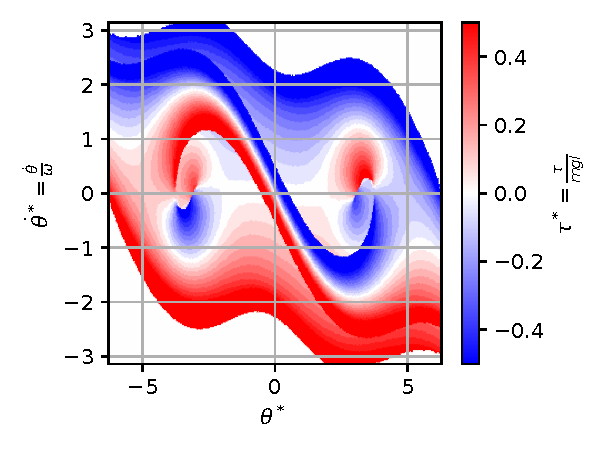
\includegraphics[width=0.90\linewidth]{fig/c1_dimpolicy.pdf}
% \caption{ 
% $\tau^*
% =
% \pi^* \left(
% \theta, \dot{\theta}^*,
% q^*=0.1 , \tau_{max}^* = 0.5
% \right)
% $
% (Context no 1, 2 and 3) 
% }\label{fig:c1_policy}
% \end{center}
% \end{figure}
% %%%%%%%%%%%%%%%%%%%%%%

% %%%%%%%%%%%%%%%%%%%%%%
% \begin{figure}[p]
% \begin{center}
% 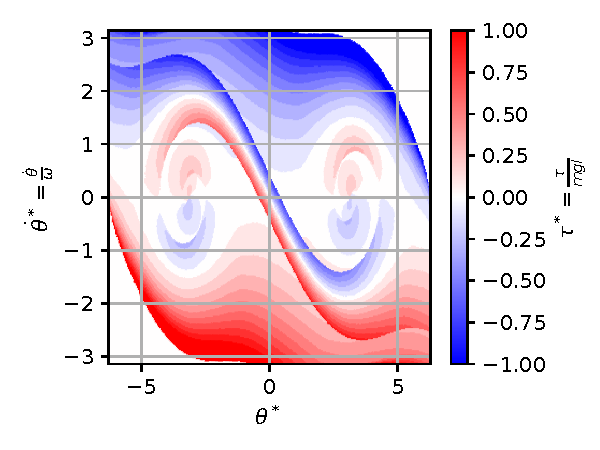
\includegraphics[width=0.90\linewidth]{fig/c4_dimpolicy.pdf}
% \caption{
% $\tau^*
% =
% \pi^* \left(
% \theta, \dot{\theta}^*,
% q^*=0.05 , \tau_{max}^* = 1.0
% \right)$
% (ontext no 4, 5 and 6)}\label{fig:c456_policy}
% \end{center}
% \end{figure}
% %%%%%%%%%%%%%%%%%%%%%%


% %%%%%%%%%%%%%%%%%%%%%%
% \begin{figure}[p]
% \begin{center}
% 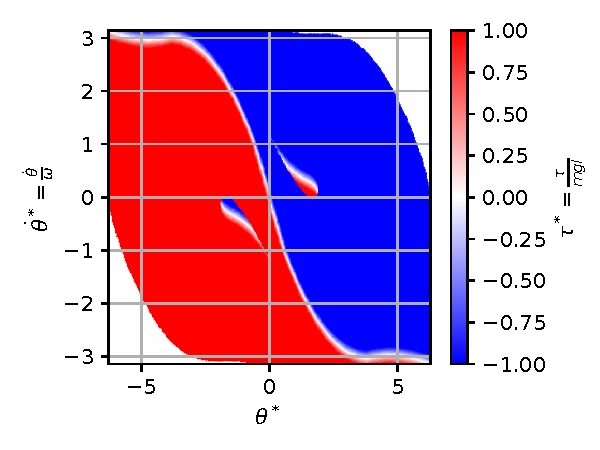
\includegraphics[width=0.90\linewidth]{fig/c7_dimpolicy.pdf}
% \caption{
% $\tau^*
% =
% \pi^* \left(
% \theta, \dot{\theta}^*,
% q^* = 10 , \tau_{max}^* = 1.0
% \right)$
% (Context no 7, 8 and 9)}\label{fig:c789_policy}
% \end{center}
% \end{figure}
% %%%%%%%%%%%%%%%%%%%%%%












% %  \begin{figure}[ht]
% %     \centering
% %     \vspace{-10pt}
% %     \subfloat[Small vehicle \label{fig:a}]{\includegraphics[width=0.12\textwidth]{fig/a.jpg}}
% %     \subfloat[Long vehicle \label{fig:b}]{\includegraphics[width=0.18\textwidth]{fig/b.jpg}}   
% %     \subfloat[Large vehicle \label{fig:c}]{\includegraphics[width=0.16\textwidth]{fig/c.PNG}}
% %     \caption{subfigures}
% %     \label{fig:subfigures}
% % \end{figure}











% %%%%%%%%%%%%%%%%%%%%%%
% \begin{figure}[p]
% \begin{center}
% 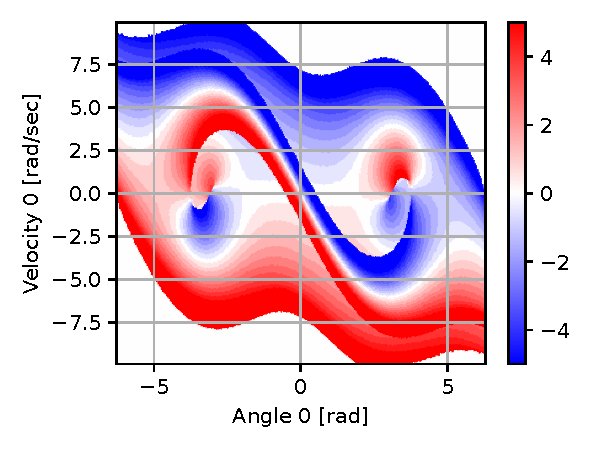
\includegraphics[width=0.99\linewidth]{fig/c1_policy.pdf}
% \caption{Context no 1 optimal policy}\label{fig:c1_policy}
% \end{center}
% \end{figure}
% %%%%%%%%%%%%%%%%%%%%%%


% %%%%%%%%%%%%%%%%%%%%%%
% \begin{figure}[p]
% \begin{center}
% 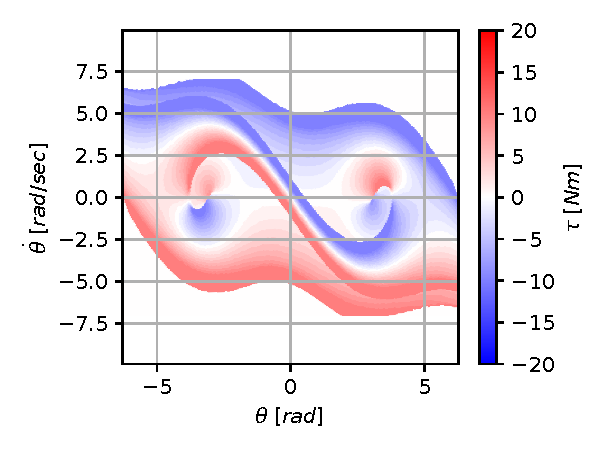
\includegraphics[width=0.99\linewidth]{fig/c2_policy.pdf}
% \caption{Context no2 optimal policy}\label{fig:c1_policy}
% \end{center}
% \end{figure}
% %%%%%%%%%%%%%%%%%%%%%%

% %%%%%%%%%%%%%%%%%%%%%%
% \begin{figure}[p]
% \begin{center}
% 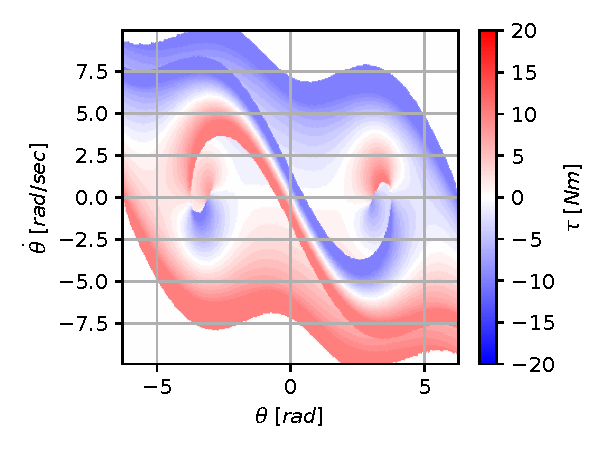
\includegraphics[width=0.99\linewidth]{fig/c3_policy.pdf}
% \caption{Context no3 optimal policy}\label{fig:c1_policy}
% \end{center}
% \end{figure}
% %%%%%%%%%%%%%%%%%%%%%%

% \newpage
% %%%%%%%%%%%%%%%%%%%%%%
% \begin{figure}[p]
% \begin{center}
% 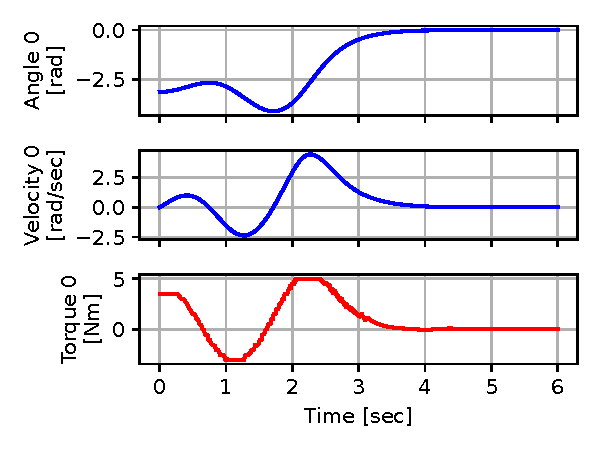
\includegraphics[width=0.99\linewidth]{fig/c1_traj.pdf}
% \caption{Context no1 optimal trajectory from up-down position}\label{fig:c1_traj}
% \end{center}
% \end{figure}
% %%%%%%%%%%%%%%%%%%%%%%


% %%%%%%%%%%%%%%%%%%%%%%
% \begin{figure}[p]
% \begin{center}
% \includegraphics[width=0.99\linewidth]{fig/c2_traj.pdf}
% \caption{Context no2 optimal trajectory from up-down position}\label{fig:c2_traj}
% \end{center}
% \end{figure}
% %%%%%%%%%%%%%%%%%%%%%%

% %%%%%%%%%%%%%%%%%%%%%%
% \begin{figure}[p]
% \begin{center}
% \includegraphics[width=0.99\linewidth]{fig/c3_traj.pdf}
% \caption{Context no3 optimal trajectory from up-down position}\label{fig:c3_traj}
% \end{center}
% \end{figure}
% %%%%%%%%%%%%%%%%%%%%%%


% %%%%%%%%%%%%%%%%%%%%%%
% \begin{figure}[p]
% \begin{center}
% \includegraphics[width=0.99\linewidth]{fig/c4_policy.pdf}
% \caption{Context no 4 optimal policy}\label{fig:c4_policy}
% \end{center}
% \end{figure}
% %%%%%%%%%%%%%%%%%%%%%%


% %%%%%%%%%%%%%%%%%%%%%%
% \begin{figure}[p]
% \begin{center}
% \includegraphics[width=0.99\linewidth]{fig/c5_policy.pdf}
% \caption{Context no5 optimal policy}\label{fig:c5_policy}
% \end{center}
% \end{figure}
% %%%%%%%%%%%%%%%%%%%%%%

% %%%%%%%%%%%%%%%%%%%%%%
% \begin{figure}[p]
% \begin{center}
% \includegraphics[width=0.99\linewidth]{fig/c6_policy.pdf}
% \caption{Context no6 optimal policy}\label{fig:c6_policy}
% \end{center}
% \end{figure}
% %%%%%%%%%%%%%%%%%%%%%%

% \newpage
% %%%%%%%%%%%%%%%%%%%%%%
% \begin{figure}[p]
% \begin{center}
% \includegraphics[width=0.99\linewidth]{fig/c4_traj.pdf}
% \caption{Context no4 optimal trajectory from up-down position}\label{fig:c4_traj}
% \end{center}
% \end{figure}
% %%%%%%%%%%%%%%%%%%%%%%


% %%%%%%%%%%%%%%%%%%%%%%
% \begin{figure}[p]
% \begin{center}
% \includegraphics[width=0.99\linewidth]{fig/c5_traj.pdf}
% \caption{Context no5 optimal trajectory from up-down position}\label{fig:c5_traj}
% \end{center}
% \end{figure}
% %%%%%%%%%%%%%%%%%%%%%%

% %%%%%%%%%%%%%%%%%%%%%%
% \begin{figure}[p]
% \begin{center}
% \includegraphics[width=0.99\linewidth]{fig/c6_traj.pdf}
% \caption{Context no6 optimal trajectory from up-down position}\label{fig:c6_traj}
% \end{center}
% \end{figure}
% %%%%%%%%%%%%%%%%%%%%%%


% %%%%%%%%%%%%%%%%%%%%%%
% \begin{figure}[p]
% \begin{center}
% \includegraphics[width=0.99\linewidth]{fig/c7_policy.pdf}
% \caption{Context no 7 optimal policy}\label{fig:c7_policy}
% \end{center}
% \end{figure}
% %%%%%%%%%%%%%%%%%%%%%%


% %%%%%%%%%%%%%%%%%%%%%%
% \begin{figure}[p]
% \begin{center}
% \includegraphics[width=0.99\linewidth]{fig/c8_policy.pdf}
% \caption{Context no8 optimal policy}\label{fig:c8_policy}
% \end{center}
% \end{figure}
% %%%%%%%%%%%%%%%%%%%%%%

% %%%%%%%%%%%%%%%%%%%%%%
% \begin{figure}[p]
% \begin{center}
% \includegraphics[width=0.99\linewidth]{fig/c9_policy.pdf}
% \caption{Context no9 optimal policy}\label{fig:c9_policy}
% \end{center}
% \end{figure}
% %%%%%%%%%%%%%%%%%%%%%%

% \newpage
% %%%%%%%%%%%%%%%%%%%%%%
% \begin{figure}[p]
% \begin{center}
% \includegraphics[width=0.99\linewidth]{fig/c7_traj.pdf}
% \caption{Context no7 optimal trajectory from up-down position}\label{fig:c7_traj}
% \end{center}
% \end{figure}
% %%%%%%%%%%%%%%%%%%%%%%


% %%%%%%%%%%%%%%%%%%%%%%
% \begin{figure}[p]
% \begin{center}
% \includegraphics[width=0.99\linewidth]{fig/c8_traj.pdf}
% \caption{Context no8 optimal trajectory from up-down position}\label{fig:c8_traj}
% \end{center}
% \end{figure}
% %%%%%%%%%%%%%%%%%%%%%%

% %%%%%%%%%%%%%%%%%%%%%%
% \begin{figure}[p]
% \begin{center}
% \includegraphics[width=0.99\linewidth]{fig/c9_traj.pdf}
% \caption{Context no9 optimal trajectory from up-down position}\label{fig:c9_traj}
% \end{center}
% \end{figure}
% %%%%%%%%%%%%%%%%%%%%%%



%%%%%%%%%%%%%%%%%%%%%%%%%%%%%%%%%%%%%%%%%%%%%%%%%%%%%%%%%%%%%%%%%%%%%%%%%%%%%%%%%%%%%%%%
\newpage
%%%%%%%%%%%%%%%%%%%%%%
\section{Closed-form parametric policies}

To better understand the concept of a dimentionless policy, here we apply the buckingham pi theorem on well-known closed form solution.

\subsection{Computed torque}

The computed torque control law provide is a model-based policy that force the system (assuming no torque limits here) on a 2nd order exponential convergence on the desired trajectory:
%%%%%%%%%%%%%%%%%%%%%%
\begin{equation}
0 = (\ddot{\theta}_d - \ddot{\theta})+ 2 \omega_d \zeta (\dot{\theta}_d - \dot{\theta}) + \omega_d^2 (\theta - \theta)
\end{equation}
%%%%%%%%%%%%%%%%%%%%%%
For the specific case of the pendulum-swing up, the desired trajectory is simply the up-right position ($\ddot{\theta}_d = \dot{\theta}_d = \theta_d = 0$), and the control law takes this form:
%%%%%%%%%%%%%%%%%%%%%%
\begin{equation}
\tau = mgl \sin \theta - 2 m l^2 \omega_d \zeta \dot{\theta} - m l^2 \omega_d^2 \theta
\label{eq:ct}
\end{equation}
%%%%%%%%%%%%%%%%%%%%%%

%%%%%%%%%%%%%%%%%%%%%%
where the only parameters are the system parameters and two variables caracterizing the convergence speed. Hence, the torque policy is a function of those variables:
%%%%%%%%%%%%%%%%%%%%%%
\begin{equation}
\underbrace{\tau}_{\text{inputs}}
=
\pi_{ct} \left(
\underbrace{ \theta, \dot{\theta} }_{\text{states}},
\underbrace{ m , g , l }_{\text{system parameters}},
\underbrace{ \omega_d , \zeta }_{\text{task parameters}}
\right)
\end{equation}
%%%%%%%%%%%%%%%%%%%%%%
having the dimension presented at table XXX.

%%%%%%%%%%%%%%%%%%%%%%%%%%%%%%%%%%%%%%%%%%%%
\begin{table}[htb]
   \centering % center the table
   \caption{Computed torque variables} 
   \label{expVari}
   \begin{tabular}{p{1.5cm} p{2.2cm} p{0.8cm} p{1.5cm} }
   \hline \hline \noalign{\smallskip} \noalign{\smallskip} \noalign{\smallskip} \noalign{\smallskip}
   %%%%%%%%%%%%%%%%%%%%%%
   \textbf{Variable} & \textbf{Description} & \textbf{Units} & \textbf{Dimensions} \\ 
   %%%%%%%%%%%%%%%%%%%%%%
   \hline \hline \noalign{\smallskip} 
   \multicolumn{4}{c}{\textbf{Control inputs}}\\ \noalign{\smallskip}  \hline \hline
   \noalign{\smallskip} 
   %%%%%%%%%%%%%%%%%%%%%%
   $\tau$ & Actuator torque & $Nm$ & [$ML^2T^{-2}$]\\ 
   %%%%%%%%%%%%%%%%%%%%%%
   \hline \hline \noalign{\smallskip} 
   \multicolumn{4}{c}{\textbf{State variables}}\\ \noalign{\smallskip}  \hline \hline \noalign{\smallskip} 
   %%%%%%%%%%%%%%%%%%%%%%
   $\theta$ & Joint angle & $rad$ & []\\ \noalign{\smallskip} \hline \noalign{\smallskip}
   $\dot{\theta}$ & Joint angular velocity & $rad/sec$ & [$T^{-1}$] \\
   %%%%%%%%%%%%%%%%%%%%%%
   \hline \hline \noalign{\smallskip} 
   \multicolumn{4}{c}{\textbf{System parameters}}\\ \noalign{\smallskip}  \hline\hline  \noalign{\smallskip} 
   %%%%%%%%%%%%%%%%%%%%%%
   $mgl$ & Maximum gravitational torque  & $Nm$ & [$ML^2T^{-2}$]  \\ \noalign{\smallskip} \hline \noalign{\smallskip}
   $\omega = \sqrt{\frac{g}{l}}$ & Natural frequency & $sec^{-1}$ & [$T^{-1}$]  \\ \noalign{\smallskip} \hline \noalign{\smallskip}
%%%%%%%%%%%%%%%%%%%%%%
   \hline \hline \noalign{\smallskip} 
   \multicolumn{4}{c}{\textbf{Policy parameters}}\\ \noalign{\smallskip}  \hline\hline  \noalign{\smallskip} 
   %%%%%%%%%%%%%%%%%%%%%%
   $\omega_d$ & Desired closed-loop frequency & $sec^{-1}$ & [$T^{-1}$]  \\ \noalign{\smallskip} \hline \noalign{\smallskip}
   $\zeta$ &  Desired closed-loop damping & $-$ & [ ]  \\ \noalign{\smallskip} \hline \noalign{\smallskip}
   \end{tabular}
\end{table}
%%%%%%%%%%%%%%%%%%%%%%%%%%%%%%%%%%%%%%%%%%%%
Here $n=7$ variables are involved and only $p=2$ independants dimensions ( $ML^2T^{-2}$ and $T^{-1}$ )
%%%%%%%%%%%%%%%%%%%%%%
\begin{equation}
m = (n = 7 ) - ( p = 2 ) = 5
\end{equation}
%%%%%%%%%%%%%%%%%%%%%%
Using $mgl$ and $\omega$, the system parameters, as the repeating variables lead to the following dimentionless groups:
%%%%%%%%%%%%%%%%%%%%%%
\begin{align}
\Pi_1 &= \tau^* = \frac{\tau}{mgl} \quad \quad \frac{[ML^2T^{-2}]}{[M][LT^{-2}][L]} \\
\Pi_2 &= \theta^* = \theta \quad \quad [-]\\
\Pi_3 &= \dot{\theta}^* = \frac{ \dot{\theta}  }{ \omega } \quad \quad \frac{[T^{-1}]}{[T^{-1}]} \\
\Pi_4 &= \omega_d^* = \frac{\omega_d}{\omega} \quad \quad \frac{[T^{-1}]}{[T^{-1}]} \\
\Pi_5 &= \zeta^* = \zeta \quad \quad []
\end{align}
%%%%%%%%%%%%%%%%%%%%%%



%%%%%%%%%%%%%%%%%%%%%%
\begin{equation}
\tau^*
=
\pi^*_{ct} \left(
\theta, \dot{\theta}^*,
\omega_d^* , \zeta^* 
\right)
\end{equation}
%%%%%%%%%%%%%%%%%%%%%%

Here we can confirme directly, dividing eq \eqref{eq:ct} by $mgl$ leads to :
%%%%%%%%%%%%%%%%%%%%%%
\begin{equation}
\tau^*
=
\sin \theta
- 2 \omega_d^* \zeta \dot{\theta}^* 
- (\omega_d^*)^2 \theta
\end{equation}
%%%%%%%%%%%%%%%%%%%%%%

% %%%%%%%%%%%%%%%%%%%%%%
% \begin{figure}[H]
% \begin{center}
% \includegraphics[width=0.99\linewidth]{fig/ct.JPG}
% \caption{Dimentionless computed torque}\label{fig:ct}
% \end{center}
% \end{figure}
% %%%%%%%%%%%%%%%%%%%%%%



%%%%%%%%%%%%%%%%%%%%%%%%%%%%%%%%%%%%%%%%%%%%%%%%%%%%%%%%%%%%%%%%%%
\newpage
\subsection{Linear Quatratic Reglator (LQR) solution}

Here we analyse the simplified control problem with the LQR framework. A linearized verison of the equation of motion is used:
%%%%%%%%%%%%%%%%%%%%%%
\begin{equation}
ml^2 \ddot{\theta} - mgl \theta = \tau
\label{eq:pendulum_dynamics}
\end{equation}
%%%%%%%%%%%%%%%%%%%%%%
Also, the same cost function that was used in section \ref{sec:optimalswingup} is used to formulate the optimal control problem:
%%%%%%%%%%%%%%%%%%%%%%
\begin{equation}
J = \int{( q^2 \theta^2 + 0 \, \dot{\theta}^2 + 1 \, \tau^2 ) dt }
\label{eq:pendulum_cost}
\end{equation}
%%%%%%%%%%%%%%%%%%%%%%
However, here no constraints on the torque are included in the problem. With this problem definition, the same variable as in section \ref{sec:optimalswingup} are presents, except the torque limit, see table \ref{tb:lqr}. The global policy solution should then have the form:
%%%%%%%%%%%%%%%%%%%%%%
\begin{equation}
\underbrace{\tau}_{\text{inputs}}
=
\pi \left(
\underbrace{ \theta, \dot{\theta} }_{\text{states}},
\underbrace{ m , g , l }_{\text{system parameters}},
\underbrace{ q }_{\text{task parameters}}
\right)
\label{eq:lqr_policy}
\end{equation}
%%%%%%%%%%%%%%%%%%%%%%
%%%%%%%%%%%%%%%%%%%%%%%%%%%%%%%%%%%%%%%%%%%%
\begin{table}[htb]
   \centering % center the table
   \caption{Pendulum swing-up optimal policy variables} 
   \label{tb:lqr}
   \begin{tabular}{p{1.2cm} p{2.5cm} p{0.8cm} p{1.5cm} }
   \hline \hline \noalign{\smallskip} \noalign{\smallskip} \noalign{\smallskip} \noalign{\smallskip}
   %%%%%%%%%%%%%%%%%%%%%%
   \textbf{Variable} & \textbf{Description} & \textbf{Units} & \textbf{Dimensions} \\ 
   %%%%%%%%%%%%%%%%%%%%%%
   \hline \hline \noalign{\smallskip} 
   \multicolumn{4}{c}{\textbf{Control inputs}}\\ \noalign{\smallskip}  \hline \hline
   \noalign{\smallskip} 
   %%%%%%%%%%%%%%%%%%%%%%
   $\tau$ & Actuator torque & $Nm$ & [$ML^2T^{-2}$]\\ 
   %%%%%%%%%%%%%%%%%%%%%%
   \hline \hline \noalign{\smallskip} 
   \multicolumn{4}{c}{\textbf{State variables}}\\ \noalign{\smallskip}  \hline \hline \noalign{\smallskip} 
   %%%%%%%%%%%%%%%%%%%%%%
   $\theta$ & Joint angle & $rad$ & []\\ \noalign{\smallskip} \hline \noalign{\smallskip}
   $\dot{\theta}$ & Joint angular velocity & $rad/sec$ & [$T^{-1}$] \\
   %%%%%%%%%%%%%%%%%%%%%%
   \hline \hline \noalign{\smallskip} 
   \multicolumn{4}{c}{\textbf{System parameters}}\\ \noalign{\smallskip}  \hline\hline  \noalign{\smallskip} 
   %%%%%%%%%%%%%%%%%%%%%%
   $mgl$ & Maximum gravitational torque  & $Nm$ & [$ML^2T^{-2}$]  \\ \noalign{\smallskip} \hline \noalign{\smallskip}
   $\omega = \sqrt{\frac{g}{l}}$ & Natural frequency & $sec^{-1}$ & [$T^{-1}$]  \\ \noalign{\smallskip} \hline \noalign{\smallskip}
%%%%%%%%%%%%%%%%%%%%%%
%%%%%%%%%%%%%%%%%%%%%%
   \hline \hline \noalign{\smallskip} 
   \multicolumn{4}{c}{\textbf{Task parameters}}\\ \noalign{\smallskip}  \hline\hline  \noalign{\smallskip} 
   %%%%%%%%%%%%%%%%%%%%%%
   $q$ & Weight parameter  & $Nm$ & [$ML^2T^{-2}$]   \\ \noalign{\smallskip} \hline \noalign{\smallskip}
   \hline \noalign{\smallskip}
   %\bottomrule[\heavyrulewidth] 
   \end{tabular}
\end{table}
%%%%%%%%%%%%%%%%%%%%%%%%%%%%%%%%%%%%%%%%%%%%
We can thus select the same dimentionless group as before, and conclude that eq. \eqref{eq:lqr_policy} can be restated under this form:
%%%%%%%%%%%%%%%%%%%%%%
\begin{equation}
\tau^*
=
\pi^* \left(
 \theta, \dot{\theta}^* ,
 q^* 
\right)
\end{equation}
%%%%%%%%%%%%%%%%%%%%%%

For this motion control problem, an analytical solution exist ( for the development, see alex screen shot 4 july 2023), and the policy is
%%%%%%%%%%%%%%%%%%%%%%
\begin{align}
\tau = 
\left[
mgl \right] \theta
+
\left[
\sqrt{ (mgl)^2 + q^2} \right] \theta
+\\
\left[
\sqrt{ 2 ml^2)} \sqrt{mgl+ \sqrt{ (mgl)^2 + q^2}}
\right] \dot{\theta}^*
\label{eq:lqr_dimpolicy}
\end{align}
%%%%%%%%%%%%%%%%%%%%%%
It is possible to, by this and that.., arrive to this dimentionless form:
%%%%%%%%%%%%%%%%%%%%%%
\begin{equation}
\tau^* = 
\left[
1 + \sqrt{ 1 + (q^*)^2}
\right] \theta
+
\left[
\sqrt{2} \sqrt{ 1 + \sqrt{ 1 + (q^*)^2}}
\right] \dot{\theta}^*
\end{equation}
%%%%%%%%%%%%%%%%%%%%%%
That correspond to the form predicted by the dimentional analysis of eq. \eqref{eq:lqr_dimpolicy}.

I am not sure where I am going with this..


%%%%%%%%%%%%%%%%%%%%%%%%%%%%%%%%%%%%%%%%%%%%%%%%%%%%%%%%%%%%%%%%%%
\newpage
\section{Conclusion}


The concept of dimentionless context is powerful, in the sense that it shows how to transfer a control policy to diferent context where the results should be exactly equivalent. However, it is limited because if the dimentionless context $c^*$ is not exactly equal, then nothing can be deduced regarding if a policy is transferable. Furthermore, the challenge of leveraging this idea is to include all meaningful context variables. If a meaningful variable (in the sense that the policy would be different if its value is changed) is omitted from the context vector $c$ in the dimentional analysis, then the dimentional analysis results might be wrong. On the other hand, if we include too many variables to fully describe a context, then dimentionnaly similar context space will probably be so specific it won't be pratical to use for transfering policy between systems. Henseforth, finding the appropriate parametrization of the context will be critical in order to leverage this principle for sharing policy between similar system, 
